\documentclass[a4paper, 12pt]{book}
%DIF LATEXDIFF DIFFERENCE FILE
%DIF DEL main-oldtmp-17776.tex   Wed Aug 29 09:49:38 2018
%DIF ADD main.tex                Wed Aug 29 09:49:33 2018
%\documentclass[a4paper, 12pt, draft]{book}  Nalogo preverite tudi z opcijo draft, ki vam bo pokazala, katere vrstice so predolge!

\usepackage[utf8x]{inputenc}   % omogoča uporabo slovenskih črk kodiranih v formatu UTF-8
\usepackage[slovene,english]{babel}    % naloži, med drugim, slovenske delilne vzorce
\usepackage[pdftex]{graphicx}  % omogoča vlaganje slik različnih formatov
\usepackage{fancyhdr}          % poskrbi, na primer, za glave strani
\usepackage{amssymb}           % dodatni simboli
\usepackage{amsmath}           % eqref, npr.
%\usepackage{hyperxmp}
\usepackage[hyphens]{url}  % dodal Solina
\usepackage{comment}       % dodal Solina

\usepackage[pdftex, colorlinks=true,
                        citecolor=black, filecolor=black, 
                        linkcolor=black, urlcolor=black,
                        pagebackref=false, 
                        pdfproducer={LaTeX}, pdfcreator={LaTeX}, hidelinks]{hyperref}

\usepackage{color}       % dodal Solina
\usepackage{soul}       % dodal Solina

\usepackage{longtable}  % dodal jaz
\usepackage{makecell}   % dodal jaz
\usepackage{minted}     % dodal jaz
\usemintedstyle{bw}     % dodal jaz

%%%%%%%%%%%%%%%%%%%%%%%%%%%%%%%%%%%%%%%%
%	DIPLOMA INFO
%%%%%%%%%%%%%%%%%%%%%%%%%%%%%%%%%%%%%%%%
\newcommand{\ttitle}{Visoko skalabilna NewSQL relacijska podatkovna baza CockroachDB}
%DIF 32c32
%DIF < \newcommand{\ttitleEn}{Higly scalable NewSQL relational database CockroachDB}
%DIF -------
\newcommand{\ttitleEn}{Higly Scalable NewSQL Relational Database CockroachDB} %DIF > 
%DIF -------
\newcommand{\tsubject}{\ttitle}
\newcommand{\tsubjectEn}{\ttitleEn}
\newcommand{\tauthor}{Matjaž Mav}
\newcommand{\tkeywords}{podatkovne baze, skaliranje, SQL, NewSQL, CockroachDB, PostgreSQL, Citus, YCSB}
\newcommand{\tkeywordsEn}{databases, scalability, SQL, NewSQL, PostgreSQL, Citus, YCSB}


%%%%%%%%%%%%%%%%%%%%%%%%%%%%%%%%%%%%%%%%
%	HYPERREF SETUP
%%%%%%%%%%%%%%%%%%%%%%%%%%%%%%%%%%%%%%%%
\hypersetup{pdftitle={\ttitle}}
\hypersetup{pdfsubject=\ttitleEn}
\hypersetup{pdfauthor={\tauthor, mm3058@student.uni-lj.si}}
\hypersetup{pdfkeywords=\tkeywordsEn}


    


%%%%%%%%%%%%%%%%%%%%%%%%%%%%%%%%%%%%%%%%
% postavitev strani
%%%%%%%%%%%%%%%%%%%%%%%%%%%%%%%%%%%%%%%%  

\addtolength{\marginparwidth}{-20pt} % robovi za tisk
\addtolength{\oddsidemargin}{40pt}
\addtolength{\evensidemargin}{-40pt}

\renewcommand{\baselinestretch}{1.3} % ustrezen razmik med vrsticami
\setlength{\headheight}{15pt}        % potreben prostor na vrhu
\renewcommand{\chaptermark}[1]%
{\markboth{\MakeUppercase{\thechapter.\ #1}}{}} \renewcommand{\sectionmark}[1]%
{\markright{\MakeUppercase{\thesection.\ #1}}} \renewcommand{\headrulewidth}{0.5pt} \renewcommand{\footrulewidth}{0pt}
\fancyhf{}
\fancyhead[LE,RO]{\sl \thepage} 
%\fancyhead[LO]{\sl \rightmark} \fancyhead[RE]{\sl \leftmark}
\fancyhead[RE]{\sc \tauthor}              % dodal Solina
\fancyhead[LO]{\sc Diplomska naloga}     % dodal Solina


\newcommand{\BibTeX}{{\sc Bib}\TeX}

%%%%%%%%%%%%%%%%%%%%%%%%%%%%%%%%%%%%%%%%
% naslovi
%%%%%%%%%%%%%%%%%%%%%%%%%%%%%%%%%%%%%%%%  


\newcommand{\autfont}{\Large}
\newcommand{\titfont}{\LARGE\bf}
\newcommand{\clearemptydoublepage}{\newpage{\pagestyle{empty}\cleardoublepage}}
\setcounter{tocdepth}{2}	      % globina kazala

%%%%%%%%%%%%%%%%%%%%%%%%%%%%%%%%%%%%%%%%
% konstrukti
%%%%%%%%%%%%%%%%%%%%%%%%%%%%%%%%%%%%%%%%  
\newtheorem{izrek}{Izrek}[chapter]
\newtheorem{trditev}{Trditev}[izrek]
\newenvironment{dokaz}{\emph{Dokaz.}\ }{\hspace{\fill}{$\Box$}}

%%%%%%%%%%%%%%%%%%%%%%%%%%%%%%%%%%%%%%%%%%%%%%%%%%%%%%%%%%%%%%%%%%%%%%%%%%%%%%%
%% PDF-A
%%%%%%%%%%%%%%%%%%%%%%%%%%%%%%%%%%%%%%%%%%%%%%%%%%%%%%%%%%%%%%%%%%%%%%%%%%%%%%%


%%%%%%%%%%%%%%%%%%%%%%%%%%%%%%%%%%%%%%%% 
% define medatata
%%%%%%%%%%%%%%%%%%%%%%%%%%%%%%%%%%%%%%%% 
\def\Title{\ttitle}
\def\Author{\tauthor, mm3058@student.uni-lj.si}
\def\Subject{\ttitleEn}
\def\Keywords{\tkeywordsEn}

%%%%%%%%%%%%%%%%%%%%%%%%%%%%%%%%%%%%%%%% 
% \convertDate converts D:20080419103507+02'00' to 2008-04-19T10:35:07+02:00
%%%%%%%%%%%%%%%%%%%%%%%%%%%%%%%%%%%%%%%% 
\def\convertDate{%
    \getYear
}

{\catcode`\D=12
    \gdef\getYear D:#1#2#3#4{\edef\xYear{#1#2#3#4}\getMonth}
}
\def\getMonth#1#2{\edef\xMonth{#1#2}\getDay}
\def\getDay#1#2{\edef\xDay{#1#2}\getHour}
\def\getHour#1#2{\edef\xHour{#1#2}\getMin}
\def\getMin#1#2{\edef\xMin{#1#2}\getSec}
\def\getSec#1#2{\edef\xSec{#1#2}\getTZh}
\def\getTZh +#1#2{\edef\xTZh{#1#2}\getTZm}
\def\getTZm '#1#2'{%
    \edef\xTZm{#1#2}%
    \edef\convDate{\xYear-\xMonth-\xDay T\xHour:\xMin:\xSec+\xTZh:\xTZm}%
}

\expandafter\convertDate\pdfcreationdate 

%%%%%%%%%%%%%%%%%%%%%%%%%%%%%%%%%%%%%%%%
% get pdftex version string
%%%%%%%%%%%%%%%%%%%%%%%%%%%%%%%%%%%%%%%% 
\newcount\countA
\countA=\pdftexversion
\advance \countA by -100
\def\pdftexVersionStr{pdfTeX-1.\the\countA.\pdftexrevision}


%%%%%%%%%%%%%%%%%%%%%%%%%%%%%%%%%%%%%%%%
% XMP data
%%%%%%%%%%%%%%%%%%%%%%%%%%%%%%%%%%%%%%%%  
\usepackage{xmpincl}
\includexmp{pdfa-1b}

%%%%%%%%%%%%%%%%%%%%%%%%%%%%%%%%%%%%%%%%
% pdfInfo
%%%%%%%%%%%%%%%%%%%%%%%%%%%%%%%%%%%%%%%%  
\pdfinfo{%
    /Title    (\ttitle)
    /Author   (\tauthor)
    /Subject  (\ttitleEn)
    /Keywords (\tkeywordsEn)
    /ModDate  (\pdfcreationdate)
    /Trapped  /False
}


%%%%%%%%%%%%%%%%%%%%%%%%%%%%%%%%%%%%%%%%%%%%%%%%%%%%%%%%%%%%%%%%%%%%%%%%%%%%%%%
%%%%%%%%%%%%%%%%%%%%%%%%%%%%%%%%%%%%%%%%%%%%%%%%%%%%%%%%%%%%%%%%%%%%%%%%%%%%%%%
%DIF PREAMBLE EXTENSION ADDED BY LATEXDIFF
%DIF UNDERLINE PREAMBLE %DIF PREAMBLE
\RequirePackage[normalem]{ulem} %DIF PREAMBLE
\RequirePackage{color}\definecolor{RED}{rgb}{1,0,0}\definecolor{BLUE}{rgb}{0,0,1} %DIF PREAMBLE
\providecommand{\DIFaddtex}[1]{{\protect\color{blue}\uwave{#1}}} %DIF PREAMBLE
\providecommand{\DIFdeltex}[1]{{\protect\color{red}\sout{#1}}}                      %DIF PREAMBLE
%DIF SAFE PREAMBLE %DIF PREAMBLE
\providecommand{\DIFaddbegin}{} %DIF PREAMBLE
\providecommand{\DIFaddend}{} %DIF PREAMBLE
\providecommand{\DIFdelbegin}{} %DIF PREAMBLE
\providecommand{\DIFdelend}{} %DIF PREAMBLE
%DIF FLOATSAFE PREAMBLE %DIF PREAMBLE
\providecommand{\DIFaddFL}[1]{\DIFadd{#1}} %DIF PREAMBLE
\providecommand{\DIFdelFL}[1]{\DIFdel{#1}} %DIF PREAMBLE
\providecommand{\DIFaddbeginFL}{} %DIF PREAMBLE
\providecommand{\DIFaddendFL}{} %DIF PREAMBLE
\providecommand{\DIFdelbeginFL}{} %DIF PREAMBLE
\providecommand{\DIFdelendFL}{} %DIF PREAMBLE
%DIF HYPERREF PREAMBLE %DIF PREAMBLE
\providecommand{\DIFadd}[1]{\texorpdfstring{\DIFaddtex{#1}}{#1}} %DIF PREAMBLE
\providecommand{\DIFdel}[1]{\texorpdfstring{\DIFdeltex{#1}}{}} %DIF PREAMBLE
\newcommand{\DIFscaledelfig}{0.5}
%DIF HIGHLIGHTGRAPHICS PREAMBLE %DIF PREAMBLE
\RequirePackage{settobox} %DIF PREAMBLE
\RequirePackage{letltxmacro} %DIF PREAMBLE
\newsavebox{\DIFdelgraphicsbox} %DIF PREAMBLE
\newlength{\DIFdelgraphicswidth} %DIF PREAMBLE
\newlength{\DIFdelgraphicsheight} %DIF PREAMBLE
% store original definition of \includegraphics %DIF PREAMBLE
\LetLtxMacro{\DIFOincludegraphics}{\includegraphics} %DIF PREAMBLE
\newcommand{\DIFaddincludegraphics}[2][]{{\color{blue}\fbox{\DIFOincludegraphics[#1]{#2}}}} %DIF PREAMBLE
\newcommand{\DIFdelincludegraphics}[2][]{% %DIF PREAMBLE
\sbox{\DIFdelgraphicsbox}{\DIFOincludegraphics[#1]{#2}}% %DIF PREAMBLE
\settoboxwidth{\DIFdelgraphicswidth}{\DIFdelgraphicsbox} %DIF PREAMBLE
\settoboxtotalheight{\DIFdelgraphicsheight}{\DIFdelgraphicsbox} %DIF PREAMBLE
\scalebox{\DIFscaledelfig}{% %DIF PREAMBLE
\parbox[b]{\DIFdelgraphicswidth}{\usebox{\DIFdelgraphicsbox}\\[-\baselineskip] \rule{\DIFdelgraphicswidth}{0em}}\llap{\resizebox{\DIFdelgraphicswidth}{\DIFdelgraphicsheight}{% %DIF PREAMBLE
\setlength{\unitlength}{\DIFdelgraphicswidth}% %DIF PREAMBLE
\begin{picture}(1,1)% %DIF PREAMBLE
\thicklines\linethickness{2pt} %DIF PREAMBLE
{\color[rgb]{1,0,0}\put(0,0){\framebox(1,1){}}}% %DIF PREAMBLE
{\color[rgb]{1,0,0}\put(0,0){\line( 1,1){1}}}% %DIF PREAMBLE
{\color[rgb]{1,0,0}\put(0,1){\line(1,-1){1}}}% %DIF PREAMBLE
\end{picture}% %DIF PREAMBLE
}\hspace*{3pt}}} %DIF PREAMBLE
} %DIF PREAMBLE
\LetLtxMacro{\DIFOaddbegin}{\DIFaddbegin} %DIF PREAMBLE
\LetLtxMacro{\DIFOaddend}{\DIFaddend} %DIF PREAMBLE
\LetLtxMacro{\DIFOdelbegin}{\DIFdelbegin} %DIF PREAMBLE
\LetLtxMacro{\DIFOdelend}{\DIFdelend} %DIF PREAMBLE
\DeclareRobustCommand{\DIFaddbegin}{\DIFOaddbegin \let\includegraphics\DIFaddincludegraphics} %DIF PREAMBLE
\DeclareRobustCommand{\DIFaddend}{\DIFOaddend \let\includegraphics\DIFOincludegraphics} %DIF PREAMBLE
\DeclareRobustCommand{\DIFdelbegin}{\DIFOdelbegin \let\includegraphics\DIFdelincludegraphics} %DIF PREAMBLE
\DeclareRobustCommand{\DIFdelend}{\DIFOaddend \let\includegraphics\DIFOincludegraphics} %DIF PREAMBLE
\LetLtxMacro{\DIFOaddbeginFL}{\DIFaddbeginFL} %DIF PREAMBLE
\LetLtxMacro{\DIFOaddendFL}{\DIFaddendFL} %DIF PREAMBLE
\LetLtxMacro{\DIFOdelbeginFL}{\DIFdelbeginFL} %DIF PREAMBLE
\LetLtxMacro{\DIFOdelendFL}{\DIFdelendFL} %DIF PREAMBLE
\DeclareRobustCommand{\DIFaddbeginFL}{\DIFOaddbeginFL \let\includegraphics\DIFaddincludegraphics} %DIF PREAMBLE
\DeclareRobustCommand{\DIFaddendFL}{\DIFOaddendFL \let\includegraphics\DIFOincludegraphics} %DIF PREAMBLE
\DeclareRobustCommand{\DIFdelbeginFL}{\DIFOdelbeginFL \let\includegraphics\DIFdelincludegraphics} %DIF PREAMBLE
\DeclareRobustCommand{\DIFdelendFL}{\DIFOaddendFL \let\includegraphics\DIFOincludegraphics} %DIF PREAMBLE
%DIF END PREAMBLE EXTENSION ADDED BY LATEXDIFF

\begin{document}
\selectlanguage{slovene}
\frontmatter
\setcounter{page}{1} %
\renewcommand{\thepage}{}       % preprecimo težave s številkami strani v kazalu
\newcommand{\sn}[1]{"`#1"'}                    % dodal Solina (slovenski narekovaji)

%%%%%%%%%%%%%%%%%%%%%%%%%%%%%%%%%%%%%%%%
%naslovnica
    \thispagestyle{empty}%
    \begin{center}
    {\large\sc Univerza v Ljubljani\\%
        Fakulteta za računalništvo in informatiko}%
    \vskip 10em%
    {\autfont \tauthor\par}%
    {\titfont \ttitle \par}%
    {\vskip 3em \textsc{DIPLOMSKO DELO\\[5mm]
    UNIVERZITETNI ŠTUDIJSKI PROGRAM\\ PRVE STOPNJE\\ RAČUNALNIŠTVO IN INFORMATIKA}\par}
    \vfill\null%
    {\large \textsc{Mentor}: izr.\ prof.\ dr.\ Matjaž Kukar\par}%
    {\vskip 2em \large Ljubljana, 2018 \par}%
\end{center}
% prazna stran
%\clearemptydoublepage      % dodal Solina (izjava o licencah itd. se izpiše na hrbtni strani naslovnice)

%%%%%%%%%%%%%%%%%%%%%%%%%%%%%%%%%%%%%%%%
%copyright stran
\thispagestyle{empty}
\vspace*{8cm}

\noindent
{\sc Copyright}. 
Rezultati \DIFdelbegin \DIFdel{diplomske naloge }\DIFdelend \DIFaddbegin \DIFadd{diplomskega dela }\DIFaddend so intelektualna lastnina avtorja in Fakultete za računalništvo in informatiko Univerze v Ljubljani.
Za objavo in koriščenje rezultatov \DIFdelbegin \DIFdel{diplomske naloge }\DIFdelend \DIFaddbegin \DIFadd{diplomskega dela }\DIFaddend je potrebno pisno privoljenje avtorja, Fakultete za računalništvo in informatiko ter mentorja.

\begin{center}
\mbox{}\vfill
\emph{Besedilo je oblikovano z urejevalnikom besedil \LaTeX.}
\end{center}
% prazna stran
\clearemptydoublepage

%%%%%%%%%%%%%%%%%%%%%%%%%%%%%%%%%%%%%%%%
% stran 3 med uvodnimi listi
\thispagestyle{empty}
\vspace*{4cm}

\noindent
Fakulteta za računalništvo in informatiko izdaja \DIFdelbegin \DIFdel{naslednjo nalogo}\DIFdelend \DIFaddbegin \DIFadd{naslednje delo}\DIFaddend :
\medskip
\begin{tabbing}
\hspace{32mm}\= \hspace{6cm} \= \kill




Tematika \DIFdelbegin \DIFdel{naloge}\DIFdelend \DIFaddbegin \DIFadd{dela}\DIFaddend :
\end{tabbing}
Besedilo teme diplomskega dela študent prepiše iz študijskega informacijskega sistema, kamor ga je vnesel mentor. V nekaj stavkih bo opisal, kaj pričakuje od kandidatovega diplomskega dela. Kaj so cilji, kakšne metode uporabiti, morda bo zapisal tudi ključno literaturo.
\vspace{15mm}






\vspace{2cm}


% prazna stran
\clearemptydoublepage


%%%%%%%%%%%%%%%%%%%%%%%%%%%%%%%%%%%%%%%%
% kazalo
\pagestyle{empty}
\def\thepage{}% preprecimo tezave s stevilkami strani v kazalu
\tableofcontents{}


% prazna stran
\clearemptydoublepage

%%%%%%%%%%%%%%%%%%%%%%%%%%%%%%%%%%%%%%%%
% seznam kratic

\chapter*{Seznam uporabljenih kratic}  % spremenil Solina, da predolge vrstice ne gredo preko desnega roba

\noindent\begin{longtable}{p{0.15\textwidth}|p{.3\textwidth}|p{.5\textwidth}}
    {\bf kratica} & {\bf angleško}
        & {\bf slovensko}
        \\ \hline
    {\bf ACID}  & atomicity, consistency, isolation, durability
        & atomarnost, konsistentnost, izolacija, trajnost so transakcijske lastnosti\DIFaddbegin \DIFadd{, }\DIFaddend katere zagotavljajo relacijske podatkovne baze
        \\
    {\bf CSV}   & comma-seperated value
        & standardni format podatkov\DIFaddbegin \DIFadd{, }\DIFaddend ločen z vejico
        \\
    {\bf DBaaS}   & database as a service
        & podatkovna baza, ki je na voljo v oblaku in s katero v večini upravlja ponudnik oblačne storitve 
        \\
    {\bf HTAP}  & hybrid transaction/analytical processing
        & oznaka sistema, ki omogoča tako transakcijsko\DIFaddbegin \DIFadd{, }\DIFaddend kakor tudi analitično obdelovanje
        \\
    {\bf IMDB}  & in-memory database
        & podatkovna baza, ki shranjuje podatke v glavni pomnilnik
        \\
    {\bf JDBC}  & Java Database Connectivity
        & javanski vmesnik za \DIFdelbegin \DIFdel{povezavanje }\DIFdelend \DIFaddbegin \DIFadd{povezovanje }\DIFaddend s podatkovnimi bazami
        \\
    {\bf JSON}  & Javascript object notation
        &  \DIFdelbegin \DIFdel{standardna }\DIFdelend \DIFaddbegin \DIFadd{standardni }\DIFaddend format za prenos podatkov v spletu\\
    {\bf KV}    & key-value
        & ključ-vrednost \\
    {\bf MVCC}    & multiversion concurrency control
        & mehanizem za nadzor sočasnosti, kateri hrani več verzij podatkov, omogoča izolacijo in konsistenco podatkov med transakcijami \\
    {\bf NewSQL}& new structured query language
        & nov strukturiran poizvedovalni jezik
        \\
    {\bf NoSQL} & not only structured query language
        & poizvedovalni jezik za delo z nerelacijskimi podatki\DIFaddbegin \DIFadd{, }\DIFaddend v nekaterih primerih tudi \DIFaddbegin \DIFadd{z }\DIFaddend relacijskimi
        \\
    {\bf NTP} & network time protocol
        & \DIFdelbegin \DIFdel{meržni }\DIFdelend \DIFaddbegin \DIFadd{mrežni }\DIFaddend protokol za sinhronizacijo ure med računalniškimi sistemi
        \\
    {\bf OLAP}  & online analytical processing
        & oznaka sistema, ki omogoča analitično obdelovanje podatkov
        \\
    {\bf OLTP}  & online transaction processing
        & oznaka sistema, ki omogoča obdelavo transakcij
        \\
    {\bf ORM}   & object-relational mapper
        & programski vmesnik za pretvorbo \DIFdelbegin \DIFdel{ralacijskih }\DIFdelend \DIFaddbegin \DIFadd{relacijskih }\DIFaddend podatkov v objekte in obratno
        \\
    {\bf SQL}   & structured query language    
        & strukturiran povpraševalni jezik za delo \DIFdelbegin \DIFdel{s }\DIFdelend \DIFaddbegin \DIFadd{z }\DIFaddend relacijskimi podatkovnimi bazami
        \\
    {\bf TPC}   & transaction processing performance council
        &  organizacija, ki se ukvarja \DIFdelbegin \DIFdel{z }\DIFdelend \DIFaddbegin \DIFadd{s }\DIFaddend primerjalno analizo podatkovnih baz v industriji
        \\
    {\bf WAL}   & write-ahead logging
        & mehanizem zabeleži najprej vse spremembe v dnevnik\DIFdelbegin \DIFdel{šele na to pa jih izvede}\DIFdelend , \DIFaddbegin \DIFadd{šele nato jih izvede; }\DIFaddend mehanizem zagotavlja atomarnost in trajnost podatkov 
        \\
    {\bf XML}   & extensible markup language
        & format za izmenjavo strukturiranih podatkov v spletu
        \\
    {\bf YCSB}  & Yahoo! Cloud Serving Benchmarking
        & enostavno orodje za izvedbo primerjalne zmogljivostne analize med različnimi podatkovnimi bazami
        \\
    {\bf 2PL} & two-phase locking
        & mehanizem za nadzor sočasnosti, kateri preko zaklepanja zagotavlja serializabilnost transakcij
        \\
\end{longtable}


% prazna stran
\clearemptydoublepage

%%%%%%%%%%%%%%%%%%%%%%%%%%%%%%%%%%%%%%%%
% povzetek
\addcontentsline{toc}{chapter}{Povzetek}
\chapter*{Povzetek}

\noindent\textbf{Naslov:} \ttitle
\bigskip

\noindent\textbf{Avtor:} \tauthor
\bigskip

%\noindent\textbf{Povzetek:} 
\noindent Diplomsko delo obravnava NewSQL podatkovno bazo CockroachDB. Cilj diplomskega dela je opisati osnovne koncepte\DIFaddbegin \DIFadd{, }\DIFaddend uporabljene v NewSQL podatkovnih bazah\DIFaddbegin \DIFadd{, }\DIFaddend in izvesti primerjalno analizo zmogljivosti med novo podatkovno bazo \DIFdelbegin \DIFdel{CockraochDB }\DIFdelend \DIFaddbegin \DIFadd{CockroachDB }\DIFaddend ter že dobro uveljavljeno podatkovno bazo PostgreSQL. NewSQL podatkovne baze so prilagojene za porazdeljena okolja in združujejo lastnosti SQL in NoSQL podatkovnih baz. Uporabljajo standardni SQL poizvedovalni jezik za interakcijo s podatkovno bazo. Preko ACID transakcij zagotavljajo visoko konsistenco podatkov. Omogočajo enostavno horizontalno skaliranje, replikacijo, visoko razpoložljivost in avtomatsko obnovo ob izpadu. Rezultati enostavnih poizvedb so pokazali, da podatkovna baza CockroachDB v primerjavi \DIFdelbegin \DIFdel{z }\DIFdelend \DIFaddbegin \DIFadd{s }\DIFaddend podatkovno bazo PostgreSQL na treh vozliščih dosega \DIFdelbegin \DIFdel{5 krat }\DIFdelend \DIFaddbegin \DIFadd{5-krat }\DIFaddend manjšo \DIFdelbegin \DIFdel{prepustnos in 3 krat }\DIFdelend \DIFaddbegin \DIFadd{prepustnost in 3-krat }\DIFaddend večjo latenco. Poleg tega pa ima \DIFdelbegin \DIFdel{trenutno }\DIFdelend podatkovna baza CockroachDB \DIFaddbegin \DIFadd{trenutno }\DIFaddend zelo slabo podporo za stične operacije.
\bigskip

\noindent\textbf{Ključne besede:} \tkeywords.
% prazna stran
\clearemptydoublepage

%%%%%%%%%%%%%%%%%%%%%%%%%%%%%%%%%%%%%%%%
% abstract
\selectlanguage{english}
\addcontentsline{toc}{chapter}{Abstract}
\chapter*{Abstract}

\noindent\textbf{Title:} \ttitleEn
\bigskip

\noindent\textbf{Author:} \tauthor
\bigskip

%\noindent\textbf{Abstract:} 
\noindent The thesis deals with \DIFaddbegin \DIFadd{a }\DIFaddend NewSQL database called CockroachDB. The aim of the thesis is to describe key concepts used in NewSQL databases and then evaluate and compare performance \DIFdelbegin \DIFdel{between }\DIFdelend \DIFaddbegin \DIFadd{of }\DIFaddend the new database CockroachDB and \DIFaddbegin \DIFadd{the }\DIFaddend well-established PostgreSQL database. NewSQL databases are \DIFdelbegin \DIFdel{build }\DIFdelend \DIFaddbegin \DIFadd{built }\DIFaddend for distributed environments and \DIFdelbegin \DIFdel{join properties from }\DIFdelend \DIFaddbegin \DIFadd{integrate the properties of }\DIFaddend both SQL and NoSQL databases. NewSQL databases use \DIFaddbegin \DIFadd{the }\DIFaddend standard SQL query language for interaction with a database. They use ACID transactions that guarantee high data consistency. They enable easier horizontal scaling, replication, high availability and automatic failover. The results of simple queries showed that CockroachDB \DIFdelbegin \DIFdel{in average achieves 3 }\DIFdelend \DIFaddbegin \DIFadd{achieves on average 5 }\DIFaddend times lower throughput and \DIFdelbegin \DIFdel{5 }\DIFdelend \DIFaddbegin \DIFadd{3 }\DIFaddend times higher latency compared to PostgreSQL \DIFaddbegin \DIFadd{on three node cluster}\DIFaddend . Furthermore, CockroachDB provides only basic support for join operations.
\bigskip

\noindent\textbf{Keywords:} \tkeywordsEn.
\selectlanguage{slovene}
% prazna stran
\clearemptydoublepage

%%%%%%%%%%%%%%%%%%%%%%%%%%%%%%%%%%%%%%%%
\mainmatter
\setcounter{page}{1}
\pagestyle{fancy}


\chapter{Uvod}
Trendi kažejo, da se vse več računalniške infrastrukture premika v oblak, s tem pa se prilagajajo in razvijajo tudi nove tehnologije, ki so temu bolj primerne. To se odraža tudi pri podatkovnih bazah. Iz starih monolitnih relacijskih podatkovnih baz, katere je še zlasti težko vzdrževati v porazdeljenih okoljih, so se razvile nerelacijske podatkovne baze in kasneje nove relacijske oziroma NewSQL podatkovne baze. NewSQL relacijske podatkovne baze so tako prilagojene za oblak. Zagotavljajo visoko konsistenco in razpoložljivost, poleg tega pa nudijo tudi boljši izkoristek računalniških virov.

Podatkovna baza CockroachDB \cite{cockroachdb/cockroach} je ena izmed NewSQL podatkovnih baz. Z raziskovalnega področja je zanimiva, ker je v celoti odprtokodna, idejno pa izhaja iz Googlove podatkovne baze Spanner \cite{spanner-home}\DIFdelbegin \DIFdel{, je }\DIFdelend \DIFaddbegin \DIFadd{. Je }\DIFaddend zelo enostavna za uporabo in je skoraj v celoti avtomatizirana. Na prvi pogled vsebuje vse, kar bi pričakovali od transakcijsko usmerjene (OLTP) podatkovne baze. 

Diplomsko delo je razdeljeno na tri večja poglavja. V prvem poglavju bomo \DIFdelbegin \DIFdel{predstavil }\DIFdelend \DIFaddbegin \DIFadd{predstavili }\DIFaddend razlog za nastanek NewSQL podatkovnih baz, opisali njihove lastnosti, razdelitev in najpogosteje uporabljene mehanizme ter pristope.

V drugem poglavju bomo opisali podatkovno bazo CockroachDB. Predstavili bomo njeno zgodovino in idejno osnovo. Poglobili se bomo v arhitekturo podatkovne baze CockroachDB in predstavili nekaj ključnih mehanizmov\DIFaddbegin \DIFadd{, }\DIFaddend kateri omogočajo standardni SQL jezik, transakcije, konsistenco, replikacijo, visoko razpoložljivost in enostavnost z upravljanjem. Kasneje bomo predstavili še ostale lastnosti\DIFaddbegin \DIFadd{, }\DIFaddend kot so SQL vmesnik, poslovna licenca ter podprta orodja, gonilniki in ORM-ji.

V tretjem poglavju bomo opisali celoten postopek izvedbe primerjalne analize zmogljivosti med podatkovno bazo CockroachDB in Citus \cite{citus}. Opisali bomo hipoteze, testno infrastrukturo, izbiro orodij za izvedbo zmogljivostnih analiz, podatkovno bazo Citus in razlog\DIFaddbegin \DIFadd{, }\DIFaddend za kaj smo CockroachDB primerjali ravno z njo, pripravo podatkov \DIFdelbegin \DIFdel{, }\DIFdelend \DIFaddbegin \DIFadd{ter }\DIFaddend izvedbo analize. Na koncu bomo predstavili rezultate \DIFaddbegin \DIFadd{ter }\DIFaddend jih komentirali.

Sledijo sklepne ugotovitve, kjer bomo \DIFdelbegin \DIFdel{povzel }\DIFdelend \DIFaddbegin \DIFadd{povzeli }\DIFaddend diplomsko delo in \DIFdelbegin \DIFdel{izpostavil }\DIFdelend \DIFaddbegin \DIFadd{izpostavili }\DIFaddend nekatere zanimive ugotovitve. Našteli bomo nekaj produktov\DIFaddbegin \DIFadd{, }\DIFaddend kjer je ta baza že v uporabi. Za zaključek bomo predlagali še nekaj odprtih vprašanj in ideje za nadaljnje raziskovanje.


\chapter{NewSQL}
NewSQL je oznaka za sodobne relacijske podatkovne baze, ki združujejo lastnosti tako relacijskih SQL, kakor tudi nerelacijskih NoSQL podatkovnih \DIFdelbegin \DIFdel{baze}\DIFdelend \DIFaddbegin \DIFadd{baz}\DIFaddend . Pojem NewSQL prvič omeni in definira Matthew Aslett aprila 2011 \cite{Pavlo2016Sep}. NewSQL podatkovne baze z relacijskih SQL podatkovnih baz prevzamejo standardni SQL vmesniki in ACID (angl. atomicity, consistency, isolation and durability) transakcijske lastnosti \cite{oliveira2017newsql}. Kratica ACID stoji za:

\begin{itemize}
    \item (A) atomarnost \DIFdelbegin \DIFdel{- }\DIFdelend \DIFaddbegin \DIFadd{– }\DIFaddend transakcija se izvede v celoti ali pa se ne izvede\DIFaddbegin \DIFadd{;
    }\DIFaddend \item (C) konsistenca \DIFdelbegin \DIFdel{- }\DIFdelend \DIFaddbegin \DIFadd{– }\DIFaddend transakcija z enega konsistentnega stanja preide v drugo konsistentno stanje\DIFaddbegin \DIFadd{;
    }\DIFaddend \item (I) izolacija \DIFdelbegin \DIFdel{- }\DIFdelend \DIFaddbegin \DIFadd{– }\DIFaddend sočasne transakcije so med seboj izolirane spremembe nepotrjenih transakcij \DIFaddbegin \DIFadd{ter }\DIFaddend niso vidne navzven\DIFaddbegin \DIFadd{;
    }\DIFaddend \item (D) trajnost \DIFdelbegin \DIFdel{- }\DIFdelend \DIFaddbegin \DIFadd{– }\DIFaddend potrjene transakcije ostanejo potrjene tudi v primeru sistemskih napak\DIFaddbegin \DIFadd{.
}\DIFaddend \end{itemize}

\noindent Z nerelacijskih NoSQL podatkovnih baz pa \DIFaddbegin \DIFadd{prevzamejo }\DIFaddend prilagojenost na porazdeljena okolja, enostavnost horizontalnega skaliranja in replikacije. NewSQL podatkovne baze nudijo primerljivo zmogljivost z NoSQL podatkovnimi bazami \cite{oliveira2017newsql}. Uporabljajo neblokirajoče mehanizme za nadzor sočasnosti \cite{NewSQLNewWayToHandleBigData}. NewSQL podatkovne baze so \DIFdelbegin \DIFdel{predvsem primerne }\DIFdelend \DIFaddbegin \DIFadd{primerne predvsem }\DIFaddend za aplikacije tipa OLTP (angl. online transaction processing) z naslednjimi lastnostmi \cite{Pavlo2016Sep}:
\begin{itemize}
    \item \DIFdelbegin \DIFdel{Izvajajo }\DIFdelend \DIFaddbegin \DIFadd{izvajajo }\DIFaddend veliko število kratkotrajnih bralno-pisalnih transakcij\DIFdelbegin \DIFdel{.
    }\DIFdelend \DIFaddbegin \DIFadd{;
    }\DIFaddend \item \DIFdelbegin \DIFdel{Večina }\DIFdelend \DIFaddbegin \DIFadd{večina }\DIFaddend transakcij preko indeksnih poizvedb uporabi le majhen del podatkov\DIFdelbegin \DIFdel{.
    }\DIFdelend \DIFaddbegin \DIFadd{;
    }\DIFaddend \item \DIFdelbegin \DIFdel{Poizvedbe }\DIFdelend \DIFaddbegin \DIFadd{poizvedbe }\DIFaddend se ponavljajo, spreminjajo pa se samo njihovi vhodni parametri.
\end{itemize}

\noindent Lastnosti NewSQL podatkovnih baz so \cite{Kumar2018Jun}:
\begin{itemize}
    \item \DIFdelbegin \DIFdel{Uporabljajo standardni SQL vmenik }\DIFdelend \DIFaddbegin \DIFadd{uporabljajo standardni SQL jezik }\DIFaddend kot primarni aplikacijski vmesnik za interakcijo\DIFdelbegin \DIFdel{.
    }\DIFdelend \DIFaddbegin \DIFadd{;
    }\DIFaddend \item \DIFdelbegin \DIFdel{Podpirajo }\DIFdelend \DIFaddbegin \DIFadd{podpirajo }\DIFaddend ACID transakcijske lastnosti\DIFdelbegin \DIFdel{.
    }\DIFdelend \DIFaddbegin \DIFadd{;
    }\DIFaddend \item \DIFdelbegin \DIFdel{Uporabljajo }\DIFdelend \DIFaddbegin \DIFadd{uporabljajo }\DIFaddend neblokirajoče mehanizme za nadzor sočasnosti. Tako pisalni zahtevki ne povzročajo konfliktov z bralnimi zahtevki \cite{NewSQLNewWayToHandleBigData}. To smo podrobneje opisali v poglavju \ref{newsql/concurrencycontroll}\DIFdelbegin \DIFdel{.
    }\DIFdelend \DIFaddbegin \DIFadd{;
    }\DIFaddend \item \DIFdelbegin \DIFdel{Implementirajo porazdeljeno }\DIFdelend \DIFaddbegin \DIFadd{implementirajo porazdeljeno in }\DIFaddend ne deljeno (angl. shared-nothing) arhitekturo. Ta arhitektura zagotavlja horizontalno skalabilnost, podatkovna baza pa lahko teče na velikem številu vozlišč brez trpljenja ozkih grl \cite{NewSQLNewWayToHandleBigData}\DIFdelbegin \DIFdel{.
    }\DIFdelend \DIFaddbegin \DIFadd{;
    }\DIFaddend \item \DIFdelbegin \DIFdel{Omogočajo }\DIFdelend \DIFaddbegin \DIFadd{omogočajo }\DIFaddend dosti boljšo zmogljivost v primerjavi \DIFdelbegin \DIFdel{z }\DIFdelend \DIFaddbegin \DIFadd{s }\DIFaddend tradicionalnimi relacijskimi podatkovnimi bazami. Nekateri pravijo, da naj bi bile NewSQL podatkovne baze celo \DIFdelbegin \DIFdel{50 krat }\DIFdelend \DIFaddbegin \DIFadd{50-krat }\DIFaddend bolj zmogljive \cite{Kumar2018Jun}.
\end{itemize}

\section{Kategorizacija NewSQL arhitektur}
Kategorizacija NewSQL podatkovnih baz deli implementacije proizvajalcev glede na njihove \DIFdelbegin \DIFdel{pristope kateri so uporabljeni}\DIFdelend \DIFaddbegin \DIFadd{uporabljene pristope}\DIFaddend , da sistem ohrani SQL vmesnik, zagotavlja skalabilnost ter zmogljivost tradicionalnih relacijskih podatkovnih baz \cite{NewSQLNewWayToHandleBigData}. NewSQL podatkovne baze se v grobem delijo na štiri kategorije \cite{Mikuletic2015Feb, Pavlo2016Sep}:

\begin{enumerate}
    \item \textbf{Nove arhitekture:}\\V to kategorijo spadajo arhitekture, katere so optimizirane za več-vozliščna porazdeljena okolja. Te arhitekture so za nas najbolj zanimive in so implementirane od začetka. Omogočajo atomično sočasnost med več-vozliščnimi sistemi, odpornost na napake preko replikacije, nadzor pretoka ter porazdeljeno procesiranje poizvedb. Slabost teh arhitektur pa je predvsem slaba kompatibilnost z obstoječimi orodji. Primeri teh arhitektur so CockroachDB \cite{cockroachdb/cockroach}, NuoDB \cite{nuodb-home}, VoltDB \cite{voltdb-home}, MemSQL \cite{memsql-home}, ... Podatkovno bazo CockroachDB smo bolj podrobno opisali v poglavju \ref{cockroachdb}.
    \item \textbf{Storitve v oblaku:}\\V to kategorijo spadajo podatkovne baze z novo arhitekturo, ki so na voljo kot produkt oziroma storitev v oblaku (DBaaS). Za upravljanje je v celoti odgovoren ponudnik oblačne storitve. Slabost te arhitekture je, da nas tipično veže na enega od ponudnikov oblačnih storitev, poleg tega pa nimamo popolnega nadzora nad delovanjem podatkovne baze. V to kategorijo na primer \DIFdelbegin \DIFdel{sodi }\DIFdelend \DIFaddbegin \DIFadd{sodijo }\DIFaddend Amazon Aurora \cite{aurora-home}, Google Spanner\cite{spanner-home}, ClearDB \cite{cleardb-home} \DIFdelbegin \DIFdel{, }\DIFdelend ...
    \item \textbf{Transparentno drobljenje:}\\To so komponente, ki usmerjajo poizvedbe, koordinirajo transakcije, upravljajo s podatki, particijami ter replikacijo. Prednost teh komponent je, da največkrat ni potrebno prilagajati aplikacije novi arhitekturi, saj še vedno deluje kot ena logična podatkovna baza. Slabost teh arhitektur pa se odraža predvsem pri neenakomerno porazdeljenih podatkih in slabi izkoriščenosti računalniških resursov. Primeri teh arhitektur so MariaDB MaxScale \cite{mariadb-maxscale-home}, ScaleArc \cite{scalearc-home}, AgilData Scalable Cluster \cite{agiledata-home} \DIFdelbegin \DIFdel{, }\DIFdelend ...
    \item \textbf{Novi shranjevalni pogoni in razširitve:}\\V to kategorijo spadajo novi shranjevalni pogoni in razširitve, kateri poizkušajo rešiti probleme skaliranja tradicionalnih relacijskih podatkovnih baz \DIFdelbegin \DIFdel{. \mbox{%DIFAUXCMD
\cite{Kumar2018Jun}}\hspace{0pt}%DIFAUXCMD
}\DIFdelend \DIFaddbegin \DIFadd{\mbox{%DIFAUXCMD
\cite{Kumar2018Jun}}\hspace{0pt}%DIFAUXCMD
. }\DIFaddend Glede na \cite{Pavlo2016Sep} te rešitve ne sodijo v svet NewSQL podatkovnih baz, ampak le med razširitve relacijskih SQL podatkovnih baz. Slabost teh v primerjavi z novimi arhitekturami je predvsem slabša izraba računalniških resursov. Poleg tega pa so arhitekture veliko manj elastične in bolj funkionalno omejene. Primeri rešitev, ki sodijo v to kategorijo\DIFaddbegin \DIFadd{, }\DIFaddend so na primer MySQL NDB cluster \cite{mysqlndbcluster-home}, Citus \cite{citus} razširitev za PostgreSQL podatkovno bazo, Hekaton \cite{hekaton-home} OLTP pogon za SQL Server \DIFdelbegin \DIFdel{, }\DIFdelend ... Podatkovno bazo Citus smo bolj podrobno opisali v poglavju \ref{benchmarking/citus}.
\end{enumerate}

\section{Nadzor sočasnosti}
\label{newsql/concurrencycontroll}
Nadzor sočasnosti je \DIFdelbegin \DIFdel{en izmen }\DIFdelend \DIFaddbegin \DIFadd{eden izmed }\DIFaddend najpomembnejših mehanizmov v podatkovnih bazah. Omogoča, da do podatkov dostopa več niti hkrati, \DIFdelbegin \DIFdel{med tem }\DIFdelend \DIFaddbegin \DIFadd{medtem }\DIFaddend pa ohranja atomičnost ter \DIFdelbegin \DIFdel{garantira }\DIFdelend \DIFaddbegin \DIFadd{jamči }\DIFaddend izolacijo \cite{Pavlo2016Sep}.

Večina NewSQL podatkovnih baz implementira varianto mehanizma z urejenimi časovnimi oznakami (angl. timestamp ordering) oziroma TO. Najbolj priljubljen je decentraliziran več-verzijski \DIFdelbegin \DIFdel{mehanizme }\DIFdelend \DIFaddbegin \DIFadd{mehanizem }\DIFaddend za nadzor so\-čas\-no\-sti (angl. multi-version concurrency control) v nadaljevanju kar MVCC \cite{Pavlo2016Sep}.
Glavna prednost MVCC mehanizma je, da omogoča sočasnost, saj bralni zahtevki nikoli ne blokirajo pisalnih in pisalni nikoli ne blokirajo bralnih. Poleg prednosti ima ta mehanizem tudi nekaj slabosti\DIFdelbegin \DIFdel{, za }\DIFdelend \DIFaddbegin \DIFadd{. Za }\DIFaddend vsako posodobitev mora shraniti novo verzijo podatka ter poskrbeti, da so zastareli podatki odstranjeni iz pomnilnika. Tako MVCC mehanizmi omogočajo večjo zmogljivost\DIFaddbegin \DIFadd{, }\DIFaddend saj so bolj prilagojeni na sočasnost, kar pa omogoča večjo izkoriščenost procesorskih virov \cite{MainMemoryDatabaseSystems}. Ključna komponenta, da MVCC mehanizem deluje v porazdeljenih okoljih, je \DIFdelbegin \DIFdel{čimbolj }\DIFdelend \DIFaddbegin \DIFadd{čim bolj }\DIFaddend točna sinhronizacija ure med vozlišči. Na primer Google Cloud Spanner uporablja posebno infrastrukturo\DIFaddbegin \DIFadd{, }\DIFaddend katera zagotavlja zelo točno sinhronizacijo ure z uporabo atomskih ur. Podatkovne baze, ki pa niso vezane na infrastrukturo, kot na primer CockroachDB, pa \DIFdelbegin \DIFdel{uporabljajo hibridne protokole }\DIFdelend za sinhronizacijo ure \DIFaddbegin \DIFadd{uporabljajo hibridne protokole }\DIFaddend \cite{Pavlo2016Sep}.

Poleg MVCC mehanizma nekatere implementacije podatkovnih baz uporabljajo kombinacijo MVCC ter dvo-fazno zaklepanje (angl. two-phase locking) oziroma 2PL \cite{Pavlo2016Sep, MainMemoryDatabaseSystems}.

\newpage

\begin{table}[H]
\begin{center}
\begin{tabular}{p{.125\textwidth}|p{.125\textwidth}|p{.65\textwidth}} 
    \textbf{T$_{\text{1}}$@1} & \textbf{T$_{\text{2}}$@2} & \textbf{komentar} \\
\hline
BEGIN  &        & T$_{\text{1}}$: začne transakcijo \\
R(A)   &        & T$_{\text{1}}$: prebere vrednost A@0 \\
W(A)   & BEGIN  & T$_{\text{1}}$: zapiše vrednost A@1; T$_{\text{2}}$: začne transakcijo \\
        & R(A)   & T$_{\text{2}}$: prebere vrednost A@0  \\
        & W(A)   & T$_{\text{2}}$: konflikt \DIFdelbeginFL \DIFdelFL{z }\DIFdelendFL \DIFaddbeginFL \DIFaddFL{s }\DIFaddendFL T$_{\text{1}}$ (čaka, da T$_{\text{1}}$ konča transakcijo) \\
R(A)   & ...    & T$_{\text{1}}$: prebere vrednost A@1; T$_{\text{2}}$: čaka \\
COMMIT & ...    & T$_{\text{1}}$: potrdi transakcijo; T$_{\text{2}}$: čaka \\
        & COMMIT & T$_{\text{2}}$: zapiše vrednost A@2 in potrdi transakcijo \\
\end{tabular}
\end{center}
\caption{Primer \cite{lecture-mvcc} konflikta, ki se zgodi ob sočasnem pisanju (W(A)) dveh transakcij T$_{\text{1}}$@1 in T$_{\text{2}}$@2 pri uporabi MVCC mehanizma. V tem primeru MVCC uporablja inkrementalne oznake\DIFaddbeginFL \DIFaddFL{, }\DIFaddendFL predstavljene z @0 @1 @2.}
\label{tbl_cc_mvcc_example}
\end{table}

\begin{table}[H]
\begin{center}
\begin{tabular}{p{.125\textwidth}|p{.125\textwidth}|p{.65\textwidth}} 
    \textbf{T$_{\text{1}}$} & \textbf{T$_{\text{2}}$} & \textbf{komentar} \\
\hline
BEGIN  &        & T$_{\text{1}}$: začne transakcijo \\
XL(A)  & BEGIN  & T$_{\text{1}}$: zahteva in pridobi ekskluzivno ključavnico nad A \\
R(A)   & SL(A)  & T$_{\text{1}}$: prebere vrednost A: T$_{\text{2}}$ zahteva deljeno ključavnico nad A (čaka, da jo T$_{\text{1}}$ sprosti) \\
W(A)   & ...    & T$_{\text{1}}$: zapiše novo vrednost A; T$_{\text{2}}$: čaka  \\
U(A)   & ...    & T$_{\text{1}}$: \DIFdelbeginFL \DIFdelFL{sporsti }\DIFdelendFL \DIFaddbeginFL \DIFaddFL{sprosti }\DIFaddendFL ključavnico nad A; T$_{\text{2}}$: čaka \\
COMMIT & R(A)    & T$_{\text{1}}$: potrdi transakcijo; T$_{\text{2}}$: pridobi deljeno ključavnico in prebere novo vrednost A \\
        & U(A)   & T$_{\text{2}}$: sprosti ključavnico nad A \\
        & COMIT  & T$_{\text{2}}$: potrdi transakcijo \\
\end{tabular}
\end{center}
\caption{Primer \cite{lecture-2pl} blokiranja, ki se zgodi ob sočasnem pisanju (W(A)) in branju (R(A)) dveh transakcij T$_{\text{1}}$ in T$_{\text{2}}$ pri uporabi 2PL protokola. Primer predpostavlja, da gre za stopnjo izolacije READ UNCOMMITED. }
\label{tbl_cc_2pl_example}
\end{table}

\section{Glavni pomnilnik}

Večina tradicionalnih relacijskih podatkovnih baz uporablja diskovno usmerjeno arhitekturo za shranjevanje podatkov. V teh sistemih je primarna lokacija za shranjevanje največkrat kar blokovno naslovljiv disk kot na primer HDD oziroma SSD. Ker so bralne in pisalne operacije v te pomnilne enote relativno počasne, se v ta namen \DIFaddbegin \DIFadd{kot predpomnilnik }\DIFaddend uporablja glavni pomnilnik \DIFdelbegin \DIFdel{kot predpomnilnik }\DIFdelend \cite{Pavlo2016Sep}.

Zgodovinsko je bil glavni pomnilnik predrag, danes pa so cene pomnilnikov nižje, tako \DIFdelbegin \DIFdel{, }\DIFdelend da v nekaterih primerih lahko celotno podatkovno bazo shranimo v glavni pomnilnik. \DIFdelbegin \DIFdel{Poslednično }\DIFdelend \DIFaddbegin \DIFadd{Posledično }\DIFaddend so tudi nekatere nove arhitekture NewSQL podatkovnih baz posvojile glavni pomnilnik kot primarno lokacijo za shranjevanje podatkov \DIFdelbegin \DIFdel{, }\DIFdelend \DIFaddbegin \DIFadd{-- }\DIFaddend te podatkovne baze označimo z IMDB (angl. in-memory database) \cite{NewSqlInMemoryAnalytics}. Glavna ideja pri tem \DIFdelbegin \DIFdel{principu }\DIFdelend \DIFaddbegin \DIFadd{načelu }\DIFaddend je, da vse podatke hranimo v glavnem pomnilniku. Poleg tega pa uporabljamo blokovno naslovljiv disk za varnostno kopiranje glavnega pomnilnika. Ta ideja izvira že iz leta 1980.
NewSQL podatkovne baze pa dodajo mehanizem, da lahko \DIFdelbegin \DIFdel{, }\DIFdelend v primeru prevelike količine podatkov \DIFdelbegin \DIFdel{, }\DIFdelend del podatkov shranijo na sekundarni pomnilnik \cite{Pavlo2016Sep}. Tako se v glavnem pomnilniku nahajajo vroči podatki \DIFdelbegin \DIFdel{, }\DIFdelend \DIFaddbegin \DIFadd{-- }\DIFaddend to so podatki\DIFaddbegin \DIFadd{, }\DIFaddend katerih se po\-iz\-ved\-be velikokrat dotaknejo, v sekundarnem pomnilniku pa se nahajajo mrzli podatki \cite{NewSqlInMemoryAnalytics}.

\DIFdelbegin \DIFdel{Tukaj }\DIFdelend \DIFaddbegin \DIFadd{Pri tem }\DIFaddend se pojavi vprašanje\DIFaddbegin \DIFadd{, }\DIFaddend kateri pristop je \DIFdelbegin \DIFdel{boljše izbrati, }\DIFdelend \DIFaddbegin \DIFadd{bolje izbrati: }\DIFaddend (1) primarno shranjevanje v glavni pomnilnik ali (2) \DIFdelbegin \DIFdel{priamrno }\DIFdelend \DIFaddbegin \DIFadd{primarno }\DIFaddend shranjevanje v blokovno naslovljivi disk z velikim glavnim pomnilnikom, kjer \DIFdelbegin \DIFdel{podatkovna baza lahko predpomni vse , }\DIFdelend \DIFaddbegin \DIFadd{lahko podatkovna baza predpomni vse }\DIFaddend oziroma skoraj vse podatke. Res je, da bo podatkovna baza pri obeh pristopih delovala bistveno hitreje. Vendar pa bo drugi pristop počasnejši od prvega, saj podatkovna baza še vedno predvideva, da se podatki nahajajo na blokovno naslovljivem disku in so nekatere operacije \DIFdelbegin \DIFdel{ne optimizirane }\DIFdelend \DIFaddbegin \DIFadd{neoptimizirane }\DIFaddend za tako delovanje \cite{garcia1992main}.

Ker glavni pomnilnik ni odporen na napake ter izpade energije, IMDB podatkovne baze uporabljajo posebne postopke, da zagotovijo obstojnost podatkov ter odpornost celotnega sistema. To dosežejo z beleženjem dogodkov v dnevnik, ki se nahaja na obstojnem pomnilniku, največkrat kar SSD. Beleženje dogodkov v dnevnik največkrat povzroči ozko grlo, zato ti sistemi poizkušajo minimizirati število teh operacij \cite{MainMemoryDatabaseSystems}. Obstaja nekaj pristopov\DIFaddbegin \DIFadd{, }\DIFaddend kako IMDB podatkovne baze beležijo dogodke v dnevnik:

\begin{itemize}
    \item \DIFdelbegin \DIFdel{Ključavnica }\DIFdelend \DIFaddbegin \DIFadd{ključavnica }\DIFaddend nad dnevnikom se odklene čim prej. S tem se zmanjša čas blokiranja ter omogoči, da se ostali dogodki hitreje zapišejo v dnevnik \cite{NewSqlInMemoryAnalytics}\DIFdelbegin \DIFdel{. 
    }\DIFdelend \DIFaddbegin \DIFadd{;
    }\DIFaddend \item \DIFdelbegin \DIFdel{Beleženje samo }\DIFdelend \DIFaddbegin \DIFadd{beleženje zgolj }\DIFaddend dogodkov, kateri spreminjajo stanje podatkov, saj so samo ti dogodki potrebni za obnovo podatkov \cite{MainMemoryDatabaseSystems}\DIFdelbegin \DIFdel{. 
    }\DIFdelend \DIFaddbegin \DIFadd{;
    }\DIFaddend \item \DIFdelbegin \DIFdel{Periodično }\DIFdelend \DIFaddbegin \DIFadd{periodično }\DIFaddend beleženje dogodkov v dnevnik. Pri tem pristopu lahko ob morebitni napaki pride do izgube transakcij \cite{NewSqlInMemoryAnalytics}\DIFdelbegin \DIFdel{.  
    }\DIFdelend \DIFaddbegin \DIFadd{;
    }\DIFaddend \item \DIFdelbegin \DIFdel{Asinhrono }\DIFdelend \DIFaddbegin \DIFadd{asinhrono }\DIFaddend potrjevanje ne čaka potrditve transakcije. Pri tem pristopu lahko ob morebitni napaki pride do izgube transakcij \cite{NewSqlInMemoryAnalytics}. 
\end{itemize}

Ker so bralne in pisalne operacije pri IMDB podatkovnih bazah, v primerjavi z tradicionalnimi relacijskimi podatkovnimi bazami, relativno veliko hitrejše, lahko te bolje izkoristijo procesorsko moč. Posledično se lahko uporabijo za poslovno analitiko na živih podatkih ter hkrati omogočajo zelo visoko pisalno prepustnost. Te procese označimo kot hibridno transakcijsko analitične procese oziroma HTAP (angl. hybrid transaction/analytical processing) \cite{NewSqlInMemoryAnalytics}.


\section{Drobljenje}
Drobljenje (angl. sharding) je pristop\DIFaddbegin \DIFadd{, }\DIFaddend s katerim večina NewSQL podatkovnih baz dosega horizontalno skalabilnost \cite{Pavlo2016Sep}. Drobljenje je vrsta horizontalnega particioniranja (angl. horizontal partitioning) podatkov, pri katerem se vsaka particija hrani na ločenem strežniku (logičnem ali fizičnem) \cite{WikiSharding}. Podatki so razdeljeni horizontalno (po vrsticah) na več delov glede na vrednosti v izbranih \DIFdelbegin \DIFdel{stolpcev }\DIFdelend \DIFaddbegin \DIFadd{stolpcih }\DIFaddend v tabeli, \DIFdelbegin \DIFdel{te stolpce }\DIFdelend \DIFaddbegin \DIFadd{katere }\DIFaddend imenujemo delitveni atributi (angl. partitioning attributes). Najbolj poznana sta dva tipa delitve:

\begin{enumerate}
    \item \textbf{Delitev glede na interval:}\\Glede na postavljene intervale se zapisi delijo na particije. Ta pristop je uporaben predvsem \DIFaddbegin \DIFadd{tam, }\DIFaddend kjer so podatki logično strukturirani v intervale, delitveni atribut pa ima veliko kardinalnost, majhno frekvenco in ni \DIFdelbegin \DIFdel{naraščujoč }\DIFdelend \DIFaddbegin \DIFadd{naraščajoč }\DIFaddend ali padajoč.
    \item \textbf{Razpršena delitev:}\\Ta delitev za delovanje uporablja razpršitveno funkcijo (angl. hash function), katera \DIFdelbegin \DIFdel{podatke }\DIFdelend poizkuša \DIFdelbegin \DIFdel{deliti čimbolj }\DIFdelend \DIFaddbegin \DIFadd{podatke deliti čim bolj }\DIFaddend enakomerno preko vseh particij.
\end{enumerate}

Idealno podatkovna baza iz poizvedbe prepozna\DIFaddbegin \DIFadd{, }\DIFaddend katerih particij se poizvedba tiče\DIFaddbegin \DIFadd{, }\DIFaddend ter nato izvede poizvedbo\DIFaddbegin \DIFadd{, }\DIFaddend porazdeljeno preko teh particij. Dobljene rezultate združi in vrne en rezultat \cite{Pavlo2016Sep}.

Nekatere izmed NewSQL podatkovnih baz omogočajo migracijo podatkov med particijami med izvajanjem podatkovne baze. Ta mehanizem je potreben, ker nekatere particije rastejo hitreje kot druge. Če želimo, da podatkovna baza deluje optimalno, \DIFdelbegin \DIFdel{potrebujemo podatke ponovno razdeliti enakomerno }\DIFdelend \DIFaddbegin \DIFadd{moramo podatke ponovno enakomerno razdeliti}\DIFaddend . Ta pristop ni nov, uporablja ga večina NoSQL podatkovnih baz, je pa bolj kompleksen, saj \DIFaddbegin \DIFadd{morajo }\DIFaddend NewSQL podatkovne baze \DIFdelbegin \DIFdel{potrebujejo }\DIFdelend zagotavljati ACID lastnosti \cite{Pavlo2016Sep}.

\section{Replikacija}

Najboljši način za doseganje visoke razpoložljivosti je uporaba replikacije. Večina sodobnih podatkovnih baz podpira nek pristop replikacije \cite{Pavlo2016Sep}. V osnovi poznamo dva pristopa repliciranja:
\begin{enumerate}
    \item \textbf{Sinhrona replikacija}:\\Imenujemo jo tudi aktivno-aktivna (angl. active-active) replikacija. Pri tem pristopu vse replike sočasno obdelajo zahtevek \cite{Pavlo2016Sep}.

    \item \textbf{Asinhrona replikacija}:\\Imenujemo jo tudi aktivno-pasivna (angl. active-passive) replikacija. Pri tem pristopu se zahtevek najprej obdela na eni repliki, nato pa se sprememba posreduje ostalim replikam. Ta pristop implementira večina NewSQL podatkovnih baz, saj zaradi ne deterministične sočas\-nosti ni mogoče izvesti zahtevkov v pravilnem vrstnem redu na vseh replikah \cite{Pavlo2016Sep, harding2017evaluation}.
\end{enumerate}

V visoko konsistentnih podatkovnih bazah morajo biti replikacija potrjene na vseh replikah, šele takrat se \DIFdelbegin \DIFdel{smatra}\DIFdelend \DIFaddbegin \DIFadd{šteje}\DIFaddend , da je replikacija uspešna \cite{NewSqlInMemoryAnalytics}. Pri porazdeljenih podatkovnih bazah, katere uporabljajo soglasni algoritem (angl. consensus algorithm), je dovolj, da replikacijo potrdi večina replik. Od soglasnih algoritmov najpogosteje zasledimo algoritma Paxos in Raft \cite{raft-vs-paxos}. Algoritem Raft je nekoliko enostavnejši za razumevanje in implementacijo ter je v porazdeljenih sistemih pogosteje uporabljen \cite{raft-vs-paxos}. 

Ker so NewSQL podatkovne baze prilagojene za oblak in namestitve\DIFaddbegin \DIFadd{, }\DIFaddend med katerimi so velike geografske razlike, podpirajo tudi optimizirano replikacijo preko WAN (angl. wide-area network) \DIFdelbegin \DIFdel{omrežji}\DIFdelend \DIFaddbegin \DIFadd{omrežij}\DIFaddend .

\section{Obnova}
Pomembna lastnost podatkovne baze, ki zagotavlja toleranco na napake, je tudi obnova podatkovne baze po izpadu. Poleg same obnove sistema, kot ga poznamo pri tradicionalnih podatkovnih bazah, NewSQL podatkovne baze  poizkušajo tudi minimizirati sam čas obnove \cite{Pavlo2016Sep}. Pričakuje se, da bo podatkovna baza na voljo skoraj ves čas, saj že kratkotrajni izpadi lahko pomenijo velike finančne izgube. Tukaj \DIFdelbegin \DIFdel{ponavadi }\DIFdelend \DIFaddbegin \DIFadd{po navadi }\DIFaddend govorimo o tako imenovanih petih devetkah (angl. five nines) oziroma 99,999 \% \DIFdelbegin \DIFdel{razpoložljivostjo, to }\DIFdelend \DIFaddbegin \DIFadd{razpoložljivosti, kar }\DIFaddend označimo \DIFdelbegin \DIFdel{z }\DIFdelend \DIFaddbegin \DIFadd{s }\DIFaddend pojmom visoka razpoložljivost.

Tradicionalne podatkovne baze \DIFdelbegin \DIFdel{ponavadi }\DIFdelend \DIFaddbegin \DIFadd{po navadi }\DIFaddend tečejo na enem vozlišču in naj\-več\-krat uporabljajo neko implementacijo algoritma ARIES (angl. Algorithms for Recovery and Isolation Exploiting Semantics) \cite{aries} za obnovo ob izpadu. ARIES za svoje delovanje uporablja WAL (angl. Write-Ahead Log)\DIFdelbegin \DIFdel{, to }\DIFdelend \DIFaddbegin \DIFadd{. To }\DIFaddend je dnevnik, ki je shranjen na obstojnem pomnilniku, vsaka sprememba pa se najprej zapiše v dnevnik in šele nato izvede. Algoritem ARIES je sestavljen iz treh faz\DIFdelbegin \DIFdel{, }\DIFdelend \DIFaddbegin \DIFadd{: }\DIFaddend analize (angl. analysis), ponovitve (angl. redo) in \DIFdelbegin \DIFdel{razveljavitev }\DIFdelend \DIFaddbegin \DIFadd{razveljavitve }\DIFaddend (angl. undo). V fazi analize algoritem pripravi podatkovne strukture. V fazi ponovitve ponovi vse spremembe, zabeležene v WAL dnevniku, v tej točki je podatkovna baza točno v takem stanju\DIFaddbegin \DIFadd{, }\DIFaddend kakor je bila pred izpadom. V fazi razveljavitve pa razveljavi vse nepotrjene transakcije. Po končanem postopku je podatkovna baza v konsistentnem stanju \DIFdelbegin \DIFdel{. \mbox{%DIFAUXCMD
\cite{Pavlo2016Sep}}\hspace{0pt}%DIFAUXCMD
}\DIFdelend \DIFaddbegin \DIFadd{\mbox{%DIFAUXCMD
\cite{Pavlo2016Sep}}\hspace{0pt}%DIFAUXCMD
.
}\DIFaddend 

Pri NewSQL podatkovnih bazah algoritem ARIES, ki ga uporabljajo tradicionalne podatkovne baze\DIFdelbegin \DIFdel{ni direktno }\DIFdelend \DIFaddbegin \DIFadd{, ni neposredno }\DIFaddend uporabljen. NewSQL podatkovne baze so porazdeljene, kar pomeni, \DIFdelbegin \DIFdel{ko eno vozlišče odpove, si }\DIFdelend \DIFaddbegin \DIFadd{da si ob odpovedi enega vozlišča }\DIFaddend ostala vozlišča avtomatsko razdelijo obremenitev, sistem kot celota pa deluje naprej. Ko pride vozlišče nazaj, mora obnoviti stanje v času izpada, poleg tega pa se mora sinhronizirati in iz ostalih vozlišč pridobiti vse spremembe, ki so se zgodile v času, ko je bilo vozlišče nedosegljivo \cite{Pavlo2016Sep}. Poleg tega je algoritem ARIES zasnovan za diskovno orientirane podatkovne baze, kar pa ni optimalno za nove pomnilniško usmerjene arhitekture NewSQL podatkovnih baz \cite{zheng2014fast}.




\chapter{CockroachDB}
\label{cockroachdb}
CockroachDB je porazdeljena SQL podatkovna baza, \DIFdelbegin \DIFdel{temelji na transakcijski in visoko konsistenti }\DIFdelend \DIFaddbegin \DIFadd{ki temelji na transakcijskem in visoko konsistentnem }\DIFaddend ključ-vrednost shranjevalnem mehanizmu. Zagotavlja ACID transakcijske lastnosti, kot primarni jezik za interakcijo pa uporablja standardni SQL. Je horizontalno skalabilna in je odporna na napake strežnika ali pa celotnega podatkovnega centra. Prilagojena je za izvajanje v \DIFdelbegin \DIFdel{oblak }\DIFdelend \DIFaddbegin \DIFadd{oblaku }\DIFaddend in namenjena globalnim oblačnim storitvam. Je transakcijska podatkovna baza in ni primerna za večje analitične obremenitve. Je zelo enostavna za upravljanje ter uporabo \DIFdelbegin \DIFdel{. \mbox{%DIFAUXCMD
\cite{CRDB-FAQ}}\hspace{0pt}%DIFAUXCMD
}\DIFdelend \DIFaddbegin \DIFadd{\mbox{%DIFAUXCMD
\cite{CRDB-FAQ}}\hspace{0pt}%DIFAUXCMD
.
}\DIFaddend 

Leta 2015 so Spencer Kimball, Ben Darnell in Peter Mattis ustanovili podjetje CockroachLabs. Njihov glavni produkt je v celoti odprtokodna podatkovna baza CockroachDB \cite{cockroachdb/cockroach}. Vsi trije ustanovitelji so bili predhodno inženirji v podjetju Google. Podatkovna baza Google Spanner pa je bila navdih za začetek podatkovne baze CockroachDB \DIFdelbegin \DIFdel{. \mbox{%DIFAUXCMD
\cite{CRDB-2017}}\hspace{0pt}%DIFAUXCMD
}\DIFdelend \DIFaddbegin \DIFadd{\mbox{%DIFAUXCMD
\cite{CRDB-2017}}\hspace{0pt}%DIFAUXCMD
.
}\DIFaddend 

Podatkovni bazi CockroachDB in Google Spanner sta si arhitekturno različni. Podatkovna baza Google Spanner deluje le v oblaku na Googlovi infrastrukturi, saj se za svoje delovanje zanaša na TrueTime API. TrueTime API je vmesnik, ki s pomočjo GPS in atomskih ur \DIFdelbegin \DIFdel{, }\DIFdelend skrbi za zelo natančno sinhronizacijo ure na Googlovi infrastrukturi \cite{Corbett:2013:SGG:2518037.2491245}. CockroachDB za svoje delovanje ne potrebuje tako točne sinhronizacije ur, v splošnem je priporočena uporaba Googlove zunanje NTP (angl. Network Time Protocol) storitve \cite{CRDB-ntpd-configuration}. Podatkovna baza CockroachDB je odprto kodna in lahko deluje v oblaku ali pa lokalno na operacijskih sistemih Linux, Windows in OS X.

\section{Arhitektura}

CockroachDB je odprtokodna, avtomatizirana, porazdeljena, skalabilna in konsistentna SQL podatkovna baza. Večino upravljanja je avtomatiziranega, kompleksnost samega sistema pa je prikrita končnemu uporabniku. 

CockroachDB v grobem sestavlja pet funkcionalnih plasti. Zaradi lažjega razumevanja večslojne arhitekture bom najprej predstavil najbolj pogoste termine in koncepte\DIFaddbegin \DIFadd{, }\DIFaddend uporabljene v podatkovni baze CockroachDB. Kasneje bom povzel samo arhitekturo in delovanje podatkovne \DIFaddbegin \DIFadd{baze}\DIFaddend , kar je bolj podrobno \DIFdelbegin \DIFdel{opisa }\DIFdelend \DIFaddbegin \DIFadd{opisano }\DIFaddend v uradni dokumentaciji \cite{CRDB-home} in prvotnih zasnutkih delovanja CockroachDB podatkovne baze \cite{CRDB-design}.

\subsubsection{Terminologija in koncepti}

\begin{itemize}
    \item \textbf{Gruča (angl. cluster):} Predstavlja en logični sistem. 
    \item \textbf{Vozlišče (angl. node):} Posamezni strežnik, ki poganja Cock\-roach\-DB, več vozlišč se poveže in tvori gručo.
    \item \textbf{Obseg (angl. range)} Nabor urejenih in sosednjih podatkov.
    \item \textbf{Replika (angl. replica):} Kopija obsega, ki se nahaja na vsaj treh vozliščih.
    \item \textbf{Najem obsega (angl. range lease):} Za vsako območje obstaja ena replika (angl. leaseholder)\DIFaddbegin \DIFadd{, }\DIFaddend katera ima obseg v najemu. Ta replika sprejme in koordinira vse bralne in pisalne zahtevke za določen obseg.
    \item \textbf{Konsistenca (angl. consistency):} Podatki v podatkovni bazi so vedno v končnem veljavnem stanju in nikoli v vmesnem stanju. Cock\-roach\-DB ohranja konsistenco preko ACID transakcij.
    \item \textbf{Soglasje (angl consensus):} To je postopek, preko katerega porazdeljeni sistemi pridejo do soglasja o vrednosti enega podatka. Podatkovna baza CockroachDB za doseganje soglasja \DIFdelbegin \DIFdel{uporabja }\DIFdelend \DIFaddbegin \DIFadd{uporablja }\DIFaddend algoritem Raft. Cock\-roach\-DB ob pisalnem zahtevku čaka, da večina replik potrditi, da je podatek uspešno zapisan. S tem mehanizmom se izognemo izgubi podatkov ter ohranimo konsistentnost podatkovne baze v primeru, da odpove eno od vozlišč.
    \item \textbf{Replikacija (angl. replication):} Je postopek kopiranja in porazdelitve podatkov med vozlišči, tako da podatki ostanejo v konsistentnem stanju. Cock\-roach\-DB uporablja sinhrono replikacijo. To pomeni, da morajo vsi pisalni zahtevki najprej dobiti soglasje \DIFdelbegin \DIFdel{kovruma}\DIFdelend \DIFaddbegin \DIFadd{kvoruma}\DIFaddend , preden se sprememba \DIFdelbegin \DIFdel{smatra }\DIFdelend \DIFaddbegin \DIFadd{šteje }\DIFaddend za potrjeno.
    \item \textbf{Transakcija (angl. transaction):} Množica \DIFdelbegin \DIFdel{operacij }\DIFdelend izvršenih \DIFaddbegin \DIFadd{operacij }\DIFaddend na podatkovni bazi, katere ohranjajo ACID lastnosti.
    \item \textbf{Visoka razpoložljivost (angl. high availability):} CockroachDB zagotavlja visoko razpoložljivost, ki ji pravimo pet devetk (angl. five nines), kar pomeni\DIFaddbegin \DIFadd{, }\DIFaddend da je sistem dosegljiv vsaj 99,999 \% časa \cite{CRDB-FAQ}.
\end{itemize}

\begin{figure}[H]
\begin{center}
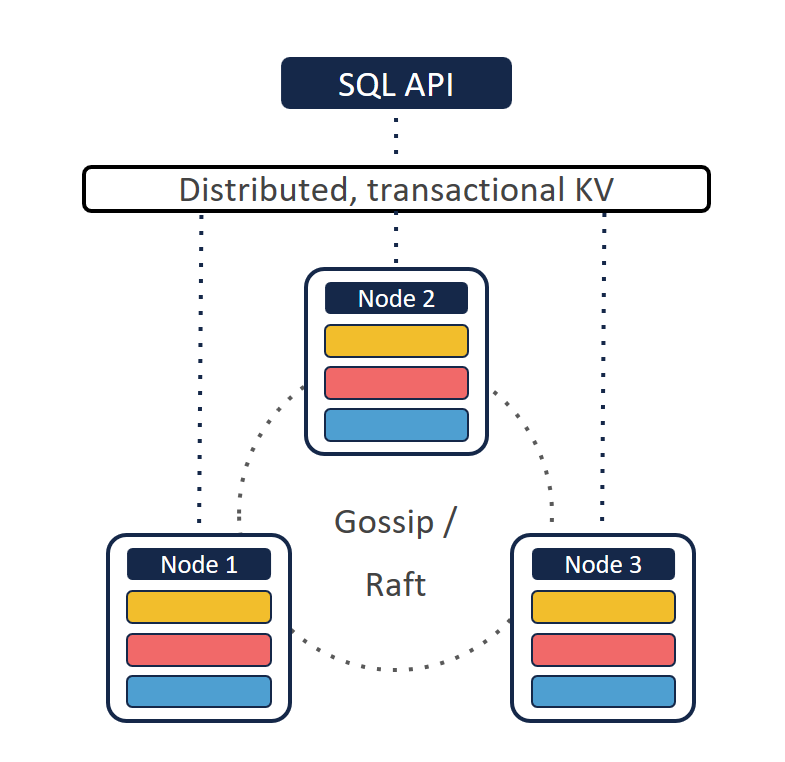
\includegraphics[width=0.5\textwidth]{resources/crdb-arhitecture-overview.png}
\end{center}
\caption{Arhitekturni pregled \cite{CRDB-2017}}
\label{img_crdb_arhitecture_overview}
\end{figure}

\subsubsection{Plasti}
Podatkovna baza CockroachDB je sestavljena iz petih plasti. Plasti med seboj delujejo kot črne škatle. Vsaka plast pa sodeluje le \DIFdelbegin \DIFdel{z plastjo direktno }\DIFdelend \DIFaddbegin \DIFadd{s plastjo neposredno }\DIFaddend nad in pod seboj.

\begin{enumerate}
    \item \textbf{SQL plast:} Prevede SQL poizvedbe v operacije tipa ključ-vrednost (KV).
    \item \textbf{Transakcijska plast:} Omogoča atomične spremembe nad večjim šte\-vi\-lom KV operacij.
    \item \textbf{Porazdelitvena plast:} Predstavi replicirana KV območja kot eno entiteto.
    \item \textbf{Replikacijska plast:} Konsistentno in sinhrono replicira KV obsege v gruči.
    \item \textbf{Shranjevalna plast:} Izvaja bralne in pisalne \DIFdelbegin \DIFdel{operacija }\DIFdelend \DIFaddbegin \DIFadd{operacije }\DIFaddend na disku.
\end{enumerate}

\subsection{SQL plast}

SQL plast predstavlja vmesnik med podatkovno bazo ter ostalimi aplikacijami.  Podatkovna baza CockroachDB implementira velik del SQL standarda \cite{CRDB-sql-standard}. Zunanje aplikacije komunicirajo preko PostgreSQL žičnega protokola (angl. PostgreSQL wire protocol) \cite{psql-wire-protocol}. To omogoča enostavno povezavo med zunanjimi aplikacijami in kompatibilnost z obstoječimi gonilniki, orodji ter ORM-ji.

Poleg tega so vsa vozlišča v CockroachDB gruči simetrična, kar pomeni, da se lahko aplikacija poveže na katero koli vozlišče. To vozlišče obdela zahtevek \DIFdelbegin \DIFdel{, }\DIFdelend oziroma ga preusmeri na vozlišče\DIFdelbegin \DIFdel{katero zna obdelati zahtevek}\DIFdelend \DIFaddbegin \DIFadd{, katero ga zna obdelati}\DIFaddend . To omogoči enostavno porazdelitev bremena.

Ko vozlišče prejme SQL zahtevek, ga najprej razčleni v abstraktno \DIFdelbegin \DIFdel{sitaksno }\DIFdelend \DIFaddbegin \DIFadd{sintaksno }\DIFaddend drevo. Potem CockroachDB začne s pripravo poizvedovalnega plana. V tem koraku CockroachDB preveri tudi semantično pravilnost poizvedb\DIFdelbegin \DIFdel{ter }\DIFdelend \DIFaddbegin \DIFadd{, }\DIFaddend nato vse operacije prevedene v KV operacije ter transformira podatke v binarno obliko. S pomočjo poizvedovalnega plana transakcijska plast nato izvede vse operacije. Kot primer poglejmo poenostavljeno stanje KV hrambe (tabela \ref{tbl_crdb_sql_kv_mapping}) po izvedbi naslednjih SQL stavkov:

\begin{listing}[H]
\begin{minted}{vim}
    \DIFdelbegin \DIFdel{CREATEA }\DIFdelend \DIFaddbegin \DIFadd{CREATE }\DIFaddend TABLE customer (
        name STRING PRIMARY KEY,
        address STRING,
        url STRING
    );
    INSERT INTO customer VALUES (
        'Apple',
        '1 Infinite Loop, Cupertino, CA',
        'http://apple.com/'
    );
\end{minted}
\label{sql-example-sql-mapping}
\end{listing}

\begin{table}[H]
\begin{center}
\begin{tabular}{ l|l } 
\textbf{ključ} & \textbf{vrednost} \\
\hline
/system/databases/mydb/id & 51 \\
/system/tables/customer/id & 42 \\ 
/system/desc/51/42/address & 69 \\ 
/system/desc/51/42/url & 66 \\
/51/42/Apple/69 & 1 Infinite Loop, Cupertino, CA \\
/51/42/Apple/66 & http://apple.com/ \\
\end{tabular}
\end{center}
\caption{Poenostavljen primer preslikave SQL v KV model \cite{CRDB-design}. V podatkovni bazi \texttt{mydb} se nahaja tabela \texttt{customer}, katera ima poleg primarnega ključa še dva stolpca \texttt{address} in \texttt{url}. Zadnja dva zapisa v tabeli predstavljata \DIFdelbeginFL \DIFdelFL{en }\DIFdelendFL \DIFaddbeginFL \DIFaddFL{eno }\DIFaddendFL vrstico v tabeli \texttt{customer} \DIFdelbeginFL \DIFdelFL{z }\DIFdelendFL \DIFaddbeginFL \DIFaddFL{s }\DIFaddendFL primarnim ključem \texttt{Apple}.}
\label{tbl_crdb_sql_kv_mapping}
\end{table}

\subsection{Transakcijska plast}
Podatkovna baza CockroachDB je konsistentna\DIFdelbegin \DIFdel{, to }\DIFdelend \DIFaddbegin \DIFadd{. To }\DIFaddend dosega tako, da transakcijska plast implementira celotno semantiko ACID transakcij. Vsak stavek je obravnavan kot svoja transakcija\DIFdelbegin \DIFdel{za katerim }\DIFdelend \DIFaddbegin \DIFadd{, za katero }\DIFaddend stoji \texttt{COMMIT}\DIFdelbegin \DIFdel{, temu }\DIFdelend \DIFaddbegin \DIFadd{. Temu }\DIFaddend pravimo način avtomatskega potrjevanja transakcij (angl. autocommit mode). Transakcije pa niso omejene samo na en stavek, določeno tabelo, obseg ali vozlišče in delujejo preko celotne gruče. To dosežejo z dvofaznim potrditvenim postopkom (angl. two-phase commit):

\begin{enumerate}
    \item \textbf{Faza 1:} Vsaka transakcija najprej kreira transakcijski zapis s statusom "v teku" (angl. pending). To je podatkovna struktura\DIFaddbegin \DIFadd{, }\DIFaddend katera nosi transakcijski ključ in status transakcije. Sočasno se za pisalne operacije kreira pisalni namen (angl. write intent). Pisalni namen je v osnovi MVCC vrednost\DIFaddbegin \DIFadd{, }\DIFaddend označena z zastavico \texttt{<intent>} in kazalcem na transakcijski zapis. Primer MVCC shrambe je prikazan v tabeli \ref{tbl_crdb_mvcc_store}.
    \item \textbf{Faza 2:} V kolikor je transakcijski zapis \DIFaddbegin \DIFadd{spremenjen }\DIFaddend v status prekinjeno (angl. aborted), se transakcija ponovno izvrši\DIFdelbegin \DIFdel{. Če }\DIFdelend \DIFaddbegin \DIFadd{, če }\DIFaddend pa so izpolnjeni vsi pogoji, se transakcija potrdi. Status v transakcijskem zapisu se spremeni v potrjeno (angl. commited).
    \item \textbf{Faza 3 (asinhrono):} Ko se transakcija konča, se vsem potrjenim pisalnim namenom odstrani zastavico \texttt{<intent>} in kazalec na transakcijski zapis. Nepotrjeni pisalni nameni se samo izbrišejo. To se izvede asinhrono, zato vse operacije, preden kreirajo pisalni namen\DIFaddbegin \DIFadd{, }\DIFaddend preverijo obstoječi pisalni namen s transakcijskim zapisom in ga ustrezno upoštevajo.
\end{enumerate}

\begin{table}[H]
\begin{center}
\begin{tabular}{ l|l|l } 
\textbf{ključ} & \textbf{čas} & \textbf{vrednost} \\
\hline
A$<$intent$>$ & 500 & nepotrjena vrednost \\
A & 400 & trenutna vrednost \\ 
A & 322 & stara vrednost \\ 
A & 50 & prvotna vrednost \\
B & 100 & vrednost B \\
\end{tabular}
\end{center}
\caption{Primer MVCC shrambe \DIFdelbeginFL \DIFdelFL{z }\DIFdelendFL \DIFaddbeginFL \DIFaddFL{s }\DIFaddendFL pisalnim namenom na ključu A \cite{CRDB-blog-transaction-isolation}.}
\label{tbl_crdb_mvcc_store}
\end{table}

Podatkovna baza CockroachDB privzeto podpira najvišji standardni SQL izolacijski nivo, to je \textit{serializable}. Ta nivo ne dopušča nikakršnih anomalij v podatkih\DIFdelbegin \DIFdel{, če }\DIFdelend \DIFaddbegin \DIFadd{. Če }\DIFaddend obstaja možnost anomalije\DIFaddbegin \DIFadd{, }\DIFaddend se transakcija ponovno izvede. Alternativno podpira tudi zastareli nestandardni izolacijski nivo \textit{snapshot}.

    
\subsection{Porazdelitvena plast}

Vsi podatki v gruči so na voljo preko \DIFdelbegin \DIFdel{kateregakoli }\DIFdelend \DIFaddbegin \DIFadd{katerega koli }\DIFaddend vozlišča. CockroachDB shranjuje podatke v urejeno vrsto tipa ključ-vrednost. Ta podatkovna stru\-ktu\-ra je namenjena shranjevanju \DIFdelbegin \DIFdel{sistemskih }\DIFdelend \DIFaddbegin \DIFadd{tako sistemskih, }\DIFaddend kakor tudi uporabniških podatkov. Z nje CockroachDB razbere\DIFaddbegin \DIFadd{, }\DIFaddend kje se nahaja podatek in vrednost samega podatka. Podatki so razdeljeni na koščke, katere imenujemo obsegi (angl. ranges). Obsegi so urejeni koščki podatkov\DIFdelbegin \DIFdel{preko katerih CockroachDB lahko }\DIFdelend \DIFaddbegin \DIFadd{, preko katerih lahko CockroachDB }\DIFaddend hitro in učinkovito izvede \textit{lookup} in \textit{scan} operacije.

Lokacija vseh obsegov je shranjena v dvo-nivojskem indeksu. Ta indeks na prvem nivoju sestavlja meta obseg (angl. meta range) imenovan \texttt{meta1}, kateri kaže na meta obseg\DIFaddbegin \DIFadd{, }\DIFaddend na drugem nivoju \DIFaddbegin \DIFadd{pa obseg, }\DIFaddend imenovan \texttt{meta2}. Meta obseg \texttt{meta2} \DIFdelbegin \DIFdel{pa }\DIFdelend kaže na podatkovne obsege.

Ko vozlišče prejme zahtevek, v meta obsegih poišče vozlišče\DIFaddbegin \DIFadd{, }\DIFaddend katero hrani obseg v najemu (angl. range lease) ter preko tega vozlišča izvede zahtevek. Meta obsegi so predpomnjeni, zato se lahko zgodi, da kažejo na napačno vozlišče. V tem primeru se vrednosti meta obsegov posodobijo.

Privzeto je velikost podatkovnega obsega omejena na \DIFdelbegin \DIFdel{64MiB}\DIFdelend \DIFaddbegin \DIFadd{64 MiB}\DIFaddend . To omogoča lažji prenos obsega med vozlišči, poleg tega pa je obseg dovolj velik, da lahko hrani nabor urejenih podatkov, kateri so bolj verjetno dostopani skupaj. Če obseg preseže velikost \DIFdelbegin \DIFdel{64MiB}\DIFdelend \DIFaddbegin \DIFadd{64 MiB}\DIFaddend , se razdeli v dva \DIFdelbegin \DIFdel{32MiB }\DIFdelend \DIFaddbegin \DIFadd{32 MiB }\DIFaddend podatkovna obsega. Ta dvo-nivojska indeksna struktura omogoča, da naslovimo do \(2^{(18 + 18)} = 2^{36}\) obsegov. Vsak obseg pa privzeto naslavlja \DIFdelbegin \DIFdel{\(2^{26}B = 64MiB\) }\DIFdelend \DIFaddbegin \DIFadd{\(2^{26}B = 64 MiB\) }\DIFaddend pomnilniške prostora. Teoretično \DIFaddbegin \DIFadd{lahko }\DIFaddend podatkovna baza CockroachDB s privzetimi nastavitvami \DIFdelbegin \DIFdel{lahko naslovi do \(2^{(36+26)}B = 4EiB\) }\DIFdelend \DIFaddbegin \DIFadd{naslovi do \(2^{(36+26)}B = 4 EiB\) }\DIFaddend podatkov. 

\subsection{Replikacijska plast}

Replikacijska plast skrbi za kopiranje podatkov med vozlišči in jih ohranja v konsistentnem stanju. To doseže preko soglasnega algoritma (angl. consensus algorithm) Raft \cite{raft-vs-paxos}. Ta algoritem zagotovi, da se večina vozlišč v gruči strinja z vsako spremembo v podatkovni bazi. S tem, kljub odpovedi posameznega vozlišča, ohrani podatke v konsistentnem stanju\DIFaddbegin \DIFadd{, }\DIFaddend poleg tega pa zagotovi nemoteno delovanje podatkovne baze (visoko razpoložljivost).

Število vozlišč, ki lahko odpove\DIFdelbegin \DIFdel{ne, }\DIFdelend \DIFaddbegin \DIFadd{, ne }\DIFaddend da bi s tem vplivalo na delovanje podatkovne baze\DIFaddbegin \DIFadd{, }\DIFaddend je enako:
\[(r - 1)/2 = f \text{, če}\ r = 3, 5, 7, ...\ \text{in}\ r <= N\]
Kjer je \(N\) število vseh vozlišč v gruči\DIFdelbegin \DIFdel{, }\DIFdelend \DIFaddbegin \DIFadd{; }\DIFaddend \(r\) faktor replikacije \DIFaddbegin \DIFadd{oz. }\DIFaddend liho število\DIFaddbegin \DIFadd{, }\DIFaddend večje ali enako tri in manjše ali enako številu vseh vozlišč v gruči\DIFdelbegin \DIFdel{. Ter }\DIFdelend \DIFaddbegin \DIFadd{; ter }\DIFaddend \(f\) maksimalno število vozlišč, ki še lahko odpove\DIFdelbegin \DIFdel{brez, }\DIFdelend \DIFaddbegin \DIFadd{, brez }\DIFaddend da bi vplivalo na delovanje podatkovne baze. Na primer če je replikacijski faktor \(r = 3\), pomeni, da za vsak obseg obstajajo 3 replike\DIFaddbegin \DIFadd{, }\DIFaddend shranjene na treh različnih vozliščih. Gruča posledično lahko tolerira odpoved enega vozlišča \(f = 1\).

Za vsak obseg obstaja Raft skupina, kjer je eno vozlišče, ki vsebuje repliko, \DIFdelbegin \DIFdel{označena }\DIFdelend \DIFaddbegin \DIFadd{označeno }\DIFaddend kot "vodja". Vodja je izvoljen in koordinira vse pisalne zahtevke za določen obseg. V idealnih pogojih je vodja Raft skupine tudi najemnik obsega (angl. leaseholder).

\subsection{Shranjevalna plast}

CockroachDB za shranjevanje uporablja KV shrambo RocksDB \cite{rocksdb-home}. Ker KV shramba RocksDB omogoča transakcije, to bistveno olajša implementacijo ACID transakcij v podatkovni bazi CockroachDB.

CockroachDB uporablja MVCC pristop in hrani več verzij vsakega podatka. Podatkovna baza CockroachDB preko MVCC pristopa omogoča poizvedbe v zgodovino \texttt{SELECT...AS OF SYSTEM TIME}. Privzeto stare verzije podatkov pretečejo po 24 urah in so počiščene iz shrambe. Primer poizvedbe po zgodovinskih podatkih:

\begin{listing}[H]
\begin{minted}{vim}
    SELECT name, balance
    FROM accounts
        AS OF SYSTEM TIME '2016-10-03 12:45:00'
    WHERE name = 'Edna Barath';
\end{minted}
\label{sql-example-as-of-system-time}
\end{listing}

\section{Lastnosti}
Razvoj podatkovne baze CockroachDB je bil usmerjen prvotno v funkcionalnosti in \DIFdelbegin \DIFdel{še le }\DIFdelend \DIFaddbegin \DIFadd{šele }\DIFaddend kasneje v optimizacije. Tako je verzija 1.0.0 (maj 2017) omogočila razvijalcem večino potrebnih funkcionalnosti\DIFaddbegin \DIFadd{, }\DIFaddend kot so poizvedovalni jezik SQL porazdeljene poizvedbe, ACID transakcije, visoka razpoložljivost preko \DIFdelbegin \DIFdel{avtomatkse }\DIFdelend \DIFaddbegin \DIFadd{avtomatske }\DIFaddend replikacije in enostavno \DIFdelbegin \DIFdel{namestitve}\DIFdelend \DIFaddbegin \DIFadd{namestitev}\DIFaddend . Verzija 2.0.0 (april 2018) pa je prinesla zmogljivostne \DIFdelbegin \DIFdel{izbolšave, }\DIFdelend \DIFaddbegin \DIFadd{izboljšave ter }\DIFaddend boljšo kompatibilnost \DIFdelbegin \DIFdel{z }\DIFdelend \DIFaddbegin \DIFadd{s }\DIFaddend podatkovno bazo PostgreSQL.

\subsection{Enostavnost}
Podatkovna baza CockroachDB stremi k enostavnosti upravljanja in vzdr\-že\-van\-ja. Večina kompleksnosti glede zagotavljanja visoke razpoložljivosti, avtomatske obnove vozlišč, usmerjanja porazdeljenih poizvedb in izenačevanja obremenitve je skoraj v celoti skrita končnemu uporabniku. Izogiba se zunanjim odvisnostim in je na voljo kot ena sama binarna datoteka. Minimalno \DIFaddbegin \DIFadd{je }\DIFaddend za zagon gruče \DIFdelbegin \DIFdel{je }\DIFdelend potrebno na vsakem vozlišču zagotoviti \DIFdelbegin \DIFdel{sinhronizacije }\DIFdelend \DIFaddbegin \DIFadd{sinhronizacijo }\DIFaddend ure, priporočena je uporaba zunanje Google NTP storitve\DIFaddbegin \DIFadd{, }\DIFaddend ter kopirati CockroachDB binarno datoteko na vsako vozlišče in jo zagnati.

\subsection{Uporabniški vmesnik in nadzorovanje}
Poleg podatkovne baze CockroachDB vsebuje tudi spletni administratorski vmesnik, ki je prikazan na sliki \ref{img_crdb_admin_ui}. Administratorski \DIFdelbegin \DIFdel{vmesniki }\DIFdelend \DIFaddbegin \DIFadd{vmesnik }\DIFaddend nudi vizualizacije raznih časovnih metrik o delovanju posameznih vozlišč, kakor tudi celotne gruče. Omogoča pregled dnevnikov in pripomore k lažjemu odkrivanju težav v gruči. CockroachDB omogoča tudi izvoz metrik v odprtokodno rešitev Prometheus, katera nam omogoča shrambo, obdelavo, vizualizacije in obveščanje nad časovnimi vrstami.

\begin{figure}[H]
\begin{center}
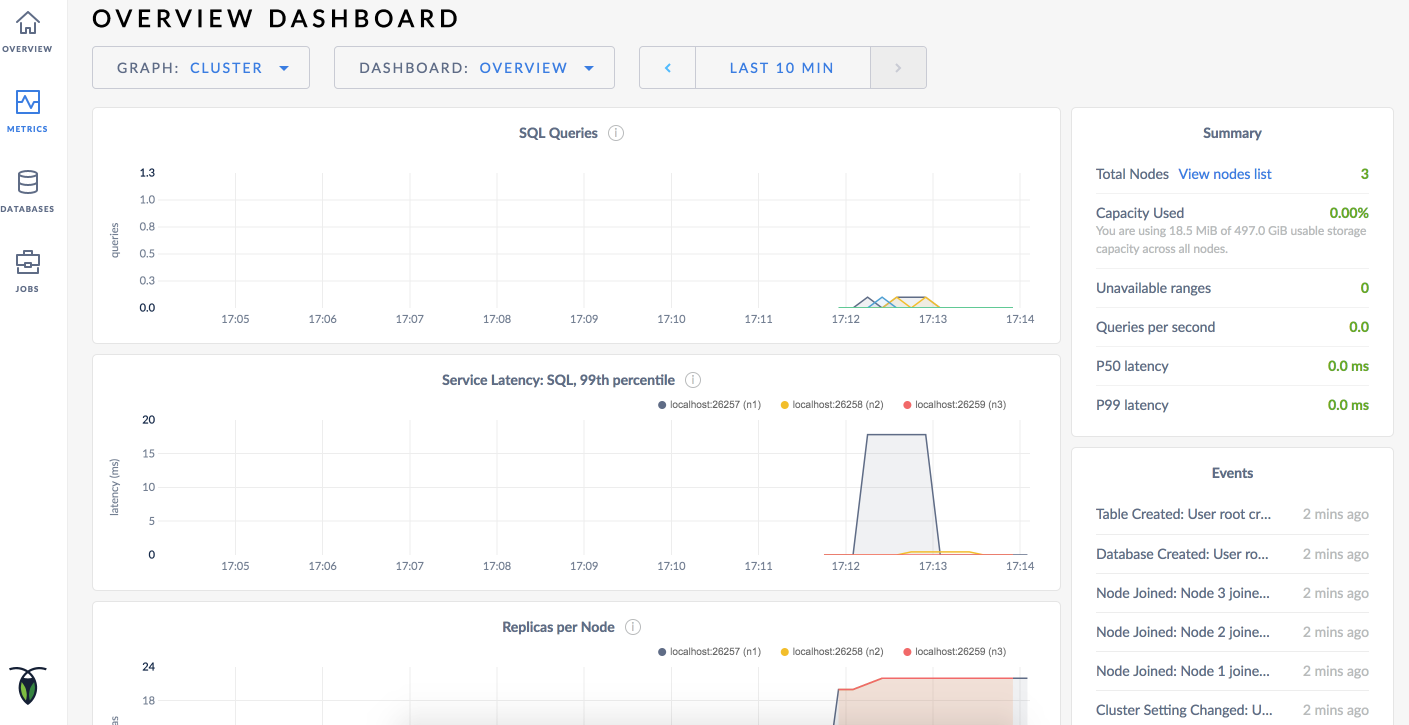
\includegraphics[width=1\textwidth]{resources/crdb_admin_ui.png}
\end{center}
\caption{Primer spletnega \DIFdelbeginFL \DIFdelFL{administratorski }\DIFdelendFL \DIFaddbeginFL \DIFaddFL{administratorskega }\DIFaddendFL vmesnika podatkovne baze CockroachDB.}
\label{img_crdb_admin_ui}
\end{figure}

\subsection{Podpora standardom SQL}
CockroachDB, kakor večina relacijskih podatkovnih baz, podpira podmnožico SQL standarda \cite{CRDB-sql-standard}. Poleg tega implementira nekatere najpogostejše raz\-ši\-rit\-ve, razširitve\DIFaddbegin \DIFadd{, }\DIFaddend specifične za PostgreSQL\DIFaddbegin \DIFadd{, }\DIFaddend ter svoje razširitve. V spodnjih podpoglavjih \DIFdelbegin \DIFdel{bom v grobem opisal}\DIFdelend \DIFaddbegin \DIFadd{bomo v grobem opisali}\DIFaddend , kaj od jezika SQL ponuja CockroachDB, bolj podroben opis pa se nahaja v uradni dokumentaciji \cite{CRDB-sql-features}.

\subsubsection{Podatkovni tipi}
CockroachDB podpira naslednje podatkovne tipe:

\begin{itemize}
    \item \textbf{Celoštevilčni}: \texttt{INT} in \texttt{SERIAL} (avtomatsko kreirana unikatna številka)
    \item \textbf{Decimalni}: \texttt{DECIMAL} in \texttt{FLOAT}
    \item \textbf{Textovni}: \texttt{STRING} in \texttt{COLLATE} (podobno kot \texttt{STRING}\DIFaddbegin \DIFadd{, }\DIFaddend vendar upošteva specifike jezika)
    \item \textbf{Datumski in časovni}: \texttt{DATE}, \texttt{TIME}, \texttt{INTERVAL} (časovni interval) in\\\texttt{TIMESTAMP} (datum in čas)
    \item \textbf{Ostali}: \texttt{ARRAY}, \texttt{BOOL}, \texttt{BYTES}, \texttt{INET} (IPv4 in IPv6 naslovi), \texttt{JSONB} in\\\texttt{UUID} (\DIFdelbegin \DIFdel{128 bitna }\DIFdelend \DIFaddbegin \DIFadd{128-bitna }\DIFaddend heksadecimalna vrednost)
\end{itemize}

\noindent Poleg zgoraj naštetih podatkovnih tipov \DIFdelbegin \DIFdel{, }\DIFdelend ima vsak podatkovni tip zaradi \DIFdelbegin \DIFdel{kompatibilnost }\DIFdelend \DIFaddbegin \DIFadd{kompatibilnosti }\DIFaddend s standardnim SQL jezikom še nekaj psevdonimov. CockroachDB ne podpira podatkovnih tipov\DIFaddbegin \DIFadd{, }\DIFaddend kot so \texttt{XML}, \texttt{UNSIGNED INT} ter \texttt{SET} in \texttt{ENUM}.

\newpage
\subsubsection{Shema}
CockroachDB podpira vse standardne ukaze za kreiranje, spreminjanje in odstranjevanje baz, tabel, stolpcev, omejitev, indeksov in pogledov. Od podatkovnih omejitev podpira vse standardne, to so: \texttt{PRIMARY KEY}, \texttt{NOT NULL}, \texttt{UNIQUE}, \texttt{CHECK}, \texttt{FOREIGN KEY} in \texttt{DEFAULT}. Omejitev \texttt{PRIMARY KEY} \DIFdelbegin \DIFdel{, }\DIFdelend lahko nastavimo samo ob kreiranju tabele in je kasneje ne moremo spreminjati. Če omejitve \texttt{PRIMARY KEY} ne nastavimo v času kreiranja tabele, CockroachDB v ozadju sam kreira skriti stolpec \DIFdelbegin \DIFdel{z }\DIFdelend \DIFaddbegin \DIFadd{s }\DIFaddend tipom \texttt{UUID}, saj je ta pomemben za samo delovanje podatkovne baze.

Poizvedovanje sheme je na voljo na standardni način, preko virtualne sheme \texttt{information\_schema}.

Prožilci (angl. triggers) še niso podprti in tudi ne načrtovani za naslednje verzije.

\subsubsection{Transakcije}
CockroachDB podpira ACID transakcije, katere so lahko porazdeljene preko celotne gruče. Privzeto transakcije uporabljajo najvišji izolacijski nivo \texttt{SERI\-ALIZABLE}, \DIFdelbegin \DIFdel{omogoča }\DIFdelend \DIFaddbegin \DIFadd{omogočajo }\DIFaddend pa še zastareli izolacijski nivo \texttt{SNAPSHOT}. Ostali standardni izolacijski nivoji niso podprti.

\subsubsection{Tabelarični izrazi}
CockroachDB podpira referenciranje tabel, pogledov, poizvedb, tabelaričnih funkcij in CTE-jev (angl. common table expressions). Podpora za CTE-je je le osnovna, referenciramo jih lahko samo enkrat\DIFaddbegin \DIFadd{, }\DIFaddend poleg tega pa jih ni mogoče uporabiti v pogledih.

Od pod-poizvedb (angl. sub-queries) omogoča le nekorelirane pod-poiz\-vedbe. Nekorelirane pod-poizvedbe so poizvedbe, katere ne referencirajo nadrejenih poizvedb. Običajno je možno korelirano pod-poizvedbo spremeniti v nekorelirano z uporabo stične operacije:

\begin{listing}[H]
\begin{minted}{vim}
    # Z \DIFdelbegin \DIFdel{uporabno }\DIFdelend \DIFaddbegin \DIFadd{uporabo }\DIFaddend korelirane pod-poizvedbe (nepodprto)
    SELECT c.name
    FROM customers c
    WHERE EXISTS(
        SELECT *
        FROM orders o
        WHERE o.customer_id = c.id
    );

    # Z uporabo stične operacije (podprto)
    SELECT DISTINCT ON(c.id) c.name
    FROM customers c CROSS JOIN orders o
    WHERE c.id = o.customer_id;
\end{minted}
\label{code-correlated-sub-queries}
\end{listing}

Od stičnih operacij CockroachDB omogoča \texttt{INNER JOIN}, \texttt{LEFT JOIN},\\\texttt{RIGHT JOIN}, \texttt{FULL JOIN} in \texttt{CROSS JOIN}. Stične operacije še niso optimizirane. Da bi \DIFdelbegin \DIFdel{le }\DIFdelend te dosegle optimalno delovanje, je zelo pomemben optimalni zapis poizvedbe, ustrezni filtri in morebitna uporaba eksperimentalne zastavice \texttt{SET experimental\_force\_lookup\_join = true}.

\subsubsection{Operatorji, skalarni izrazi, logični izrazi in funkcije}
CockroachDB implementira večji del standardnih operatorjev, skalarnih izrazov, logičnih izrazov ter funkcij. Podpira poizvedovanje po tipu JSON, omogoča iskanje \DIFdelbegin \DIFdel{z }\DIFdelend \DIFaddbegin \DIFadd{s }\DIFaddend POSIX regularnimi izrazi ter implementira agregacijske funkcije (funkcije\DIFaddbegin \DIFadd{, }\DIFaddend katere se izvedejo nad posamezno skupino ob uporabi \texttt{GROUP BY}) in okenske funkcije (\texttt{OVER()}).

Uporabniške funkcije niso podprte in tudi ne načrtovane za naslednje verzije. Shranjene procedure so načrtovane za eno od naslednjih verzij.

\subsection{Licenca}

CockroachDB je odprtokodna in zastonjska podatkovna baza. \DIFdelbegin \DIFdel{Večina }\DIFdelend \DIFaddbegin \DIFadd{Večino }\DIFaddend potrebnih funkcionalnosti omogoča zastonjska različica, poleg tega pa ponuja tudi poslovno licenco. Poslovna licenca \DIFdelbegin \DIFdel{omogoča strankam }\DIFdelend \DIFaddbegin \DIFadd{strankam omogoča}\DIFaddend :

\begin{itemize}
    \item svetovanje\DIFdelbegin \DIFdel{,
    }\DIFdelend \DIFaddbegin \DIFadd{;
    }\DIFaddend \item tehnično pomoč\DIFdelbegin \DIFdel{,
    }\DIFdelend \DIFaddbegin \DIFadd{;
    }\DIFaddend \item geografsko porazdelitev podatkov na nivoju ene vrstice (podatki so blizu uporabnika)\DIFdelbegin \DIFdel{, 
    }\DIFdelend \DIFaddbegin \DIFadd{;
    }\DIFaddend \item vizualizacijo geografsko porazdelitve gruče na zemljevidu\DIFdelbegin \DIFdel{,
    }\DIFdelend \DIFaddbegin \DIFadd{;
    }\DIFaddend \item nadzor dostopa na nivoju skupin in
    \item porazdeljeno kreiranje in \DIFdelbegin \DIFdel{obnova }\DIFdelend \DIFaddbegin \DIFadd{obnovo }\DIFaddend varnostnih kopij.
\end{itemize}

\subsection{Podprta orodja, gonilniki\DIFdelbegin \DIFdel{in }\DIFdelend \DIFaddbegin \DIFadd{, }\DIFaddend ORM-ji in skupnost}

Podatkovna baza CockroachDB implementira standardni SQL \cite{CRDB-sql-standard}, za komunikacijo med odjemalcem in strežnikom pa uporablja PostgreSQL žični protokol, kar omogoča dobro kompatibilnost z obstoječimi PostgreSQL komponentami.

Na uradni spletni dokumentaciji je za jezike Go, Java, .NET, C++, NodeJS, PHP, Python, Ruby, Rust, Clojure ter Elixir objavljen seznam podprtih gonilnikov in ORM-jev. Za vse gonilnike CockroachLabs v času pisanja zagotavlja le beta podporo \cite{CRDB-meta-drivers-orms}.

Od orodij za upravljanje \DIFdelbegin \DIFdel{z }\DIFdelend \DIFaddbegin \DIFadd{s }\DIFaddend podatkovno bazo nam CockroachLabs ponuja konzolno aplikacijo \texttt{cockroach sql}. Od grafičnih orodij nudijo beta podporo \cite{CRDB-meta-vizualizers} za pgweb \cite{pgweb-home}, dbglass \cite{dbglass-home}, Postico \cite{postico-home}, PSequel \cite{psequel-home}, TablePlus \cite{tableplus-home} in Valentina studio \cite{valentinastudio-home}.

Orodje pgweb, \DIFdelbegin \DIFdel{katero }\DIFdelend \DIFaddbegin \DIFadd{ki }\DIFaddend je bilo primarno razvito za podatkovno bazo PostgreSQL, ima trenutno najbolj aktivno skupnost, je odprtokodno in podpira vse glavne operacijske sisteme (Windows, OSX in Linux). Do aplikacije dostopamo preko spletnega brskalnika. Orodje pgweb podpira funkcionalnosti\DIFaddbegin \DIFadd{, }\DIFaddend kot so:

\begin{itemize}
    \item pregled podatkovne baze in sheme\DIFaddbegin \DIFadd{;
    }\DIFaddend \item izvedba in analiza SQL poizvedb\DIFaddbegin \DIFadd{;
    }\DIFaddend \item zgodovina poizvedb\DIFaddbegin \DIFadd{;
    }\DIFaddend \item izvoz podatkov v formatu CSV, JSON in XML\DIFaddbegin \DIFadd{.
}\DIFaddend \end{itemize}

Izvirna koda podatkovne baze CockroachDB je javno dostopna preko GitHub repozitorija \texttt{cockroachdb/cockraoch} \cite{cockroachdb/cockroach}. Projekt ima aktivno skupnost \DIFdelbegin \DIFdel{, kateremu }\DIFdelend \DIFaddbegin \DIFadd{in mu }\DIFaddend trenutno sledi približno 14 tisoč navdušencev. Poleg GitHub repozitorija, kjer se odvija ves razvoj, vodenje nalog in pomoč, CockroachLabs vodi še spletno stran \cite{CRDB-home} (dokumentacija, form, blog, mediji), Gitter kanal \cite{CRDB-gitter} in Docker repozitorij \cite{CRDB-docker}.

\chapter{Primerjalna analiza zmogljivosti CockroachDB}

Primerjalna analiza zmogljivosti (angl. performance benchmarking) je postopek za primerjavo enega sistema z ostalimi podobnimi sistemi. V našem primeru smo z orodjem YCSB primerjali podatkovni bazi CockroachDB ter PostgreSQL z nameščeno razširitvijo Citus (v nadaljevanju samo Citus). 

Za primerjavo \DIFdelbegin \DIFdel{z }\DIFdelend \DIFaddbegin \DIFadd{s }\DIFaddend Citus smo se odločil zaradi lažje izvedbe ter bolj primerljivih rezultatov. Obe podatkovni bazi CockroachDB in Citus sta po nekaterih lastnostih zelo podobni. Obe podatkovni bazi \DIFdelbegin \DIFdel{implementirat }\DIFdelend \DIFaddbegin \DIFadd{implementirata }\DIFaddend standardni SQL ter komunicirata preko PostgreSQL žičnega protokola. Podatkovno bazo smo nekoliko bolj podrobno opisali v poglavju \ref{benchmarking/citus}.

Za orodje YCSB smo se odločili, saj podpira vmesnik JDBC, katerega podpirata tudi obe podatkovni bazi\DIFaddbegin \DIFadd{, }\DIFaddend poleg tega pa je \DIFdelbegin \DIFdel{enostaven }\DIFdelend \DIFaddbegin \DIFadd{enostavno }\DIFaddend za uporabo. Orodje YCSB smo bolj podrobno opisal v poglavju \ref{YCSB_about}. Ob iskanju najprimernejšega orodja smo pregledali še naslednja orodja:

\begin{itemize}
    \item \textbf{TPC:}\\ TPC (angl. transaction processing performance council) \cite{TPC-home} je \DIFdelbegin \DIFdel{ne profitna organizacija, katera }\DIFdelend \DIFaddbegin \DIFadd{neprofitna organizacija, ki }\DIFaddend nudi preverljive podatke TPC zmogljivostnih analiz podatkovnih baz. TPC definira več različnih standardnih testov, \DIFdelbegin \DIFdel{kateri }\DIFdelend \DIFaddbegin \DIFadd{ki }\DIFaddend simulirajo različne realne obremenitve. \DIFdelbegin \DIFdel{Te testi so točno }\DIFdelend \DIFaddbegin \DIFadd{Ti testi so natančno }\DIFaddend opisani, strogo omejeni in kompleksni. Primer testa za transakcijske obremenitve je test TPC-C\DIFdelbegin \DIFdel{kateri }\DIFdelend \DIFaddbegin \DIFadd{, ki }\DIFaddend simulira obremenitve v dobavnem skladišču. Primer za testiranje analitičnih \DIFdelbegin \DIFdel{obremenitve }\DIFdelend \DIFaddbegin \DIFadd{obremenitev }\DIFaddend je test TPC-H\DIFdelbegin \DIFdel{kateri }\DIFdelend \DIFaddbegin \DIFadd{, ki }\DIFaddend izvaja kompleksne poizvedbe za podporo pri odločanju.

    TPC testi so standardizirani in simulirajo realne obremenitve za dolo\-čene problemske domene. \DIFdelbegin \DIFdel{Te }\DIFdelend \DIFaddbegin \DIFadd{Ti }\DIFaddend testi bi bili najbolj primerni, vendar pa so zelo točno definirani, kompleksni in težki za izvedbo, zato jih v \DIFdelbegin \DIFdel{diplomski nalogi }\DIFdelend \DIFaddbegin \DIFadd{diplomskem delu }\DIFaddend nismo izvedli. Uradnih TPC testov za podatkovno bazo CockroachDB še ni.
    \item \textbf{pgbench:}\\ Je enostavno orodje\DIFaddbegin \DIFadd{, }\DIFaddend namenjeno zmogljivostni analizi PostgreSQL podatkovnih baz \cite{pgbench}. Simulira transakcijsko obremenitev, podobno zastarelemu testu TPC-B. Test TPC-B simulira obremenitve v bančni\-štvu. 

    Orodje pgbench v času testiranja še ni bilo kompatibilno \DIFdelbegin \DIFdel{z }\DIFdelend \DIFaddbegin \DIFadd{s }\DIFaddend podatkovno bazo CockroachDB.
    \item \textbf{cockroachdb/loadgen:}\\ Je skupek \DIFdelbegin \DIFdel{orodj }\DIFdelend \DIFaddbegin \DIFadd{orodij, }\DIFaddend namenjenih zmogljivostni analizi CockroachDB podatkovne baze \cite{cockroachdb/loadgen}. Orodje vsebuje nabor testov, ki generirajo TPC-C, TPC-H, YCSB in KV obremenitve. Te orodja CockroachLabs interno uporablja za zmogljivostno primerjavo med posameznimi verzijami podatkovne baze CockroachDB. Kasneje je bil objavljen članek, kjer so primerjali rezultate TPC-C obremenitve med podatkovnima bazama CockroachDB in Amazon Aurora \cite{CRDB-tpcc-vs-aurora}.

    Orodje je enostavno, vendar pa je slabo dokumentirano in ne omogoča zmogljivostne analize podatkovne baze PostgreSQL.
    \item \textbf{Apache JMeter:}\\ Je orodje\DIFaddbegin \DIFadd{, }\DIFaddend namenjeno izvajanju raznih obremenitvenih testov \cite{jmeter}. Orod\-je omogoča izvajanje poljubnih obremenitev podatkovnih baz preko JDBC vmesnika.

    Orodje je zelo konfigurabilno\DIFaddbegin \DIFadd{, }\DIFaddend vendar pa ne omogoča v naprej definiranih obremenitvenih testov. Zaradi kompleksnosti je težko za uporabo.
    \item \textbf{YCSB:}\\ YCSB (angl. Yahoo! Cloud Serving Benchmark) je orodje\DIFaddbegin \DIFadd{, }\DIFaddend namenjeno za primerjavo zmogljivostnih metrik med raznimi podatkovnimi bazami \cite{brianfrankcooper/YCSB}. Orodje smo podrobneje opisali v poglavju \ref{YCSB_about}.
\end{itemize}

V naslednjih podpoglavjih bomo opisali točen postopek\DIFaddbegin \DIFadd{, }\DIFaddend s katerim smo izvedli primerjalno analizo. Opisali bomo strojno arhitekturo, pripravo posameznih konfiguracij, pripravo podatkov in samo testiranje. Na koncu bomo predstavili rezultate zmogljivostne analize ter naše ugotovitve.

\section{Hipoteze}
Pred začetkom izvajanja primerjalne analize smo postavili naslednje hipoteze:
\begin{enumerate}
    \item CockroachDB bo na enem vozlišču nekoliko počasnejši od PostgreSQL podatkovne baze.
    \iffalse
    Razlog za to hipotezo je, da je CockroachDB na trgu dobro leto in še ni dokončno \DIFdelbegin \DIFdel{optimizirana. Medtem, }\DIFdelend \DIFaddbegin \DIFadd{optimiziran, medtem }\DIFaddend ko je PostgreSQL na trgu dobrih 20 let.
    \fi
    \item CockroachDB bo zaradi linearne skalabilnosti na treh vozliščih skoraj \DIFdelbegin \DIFdel{tri krat }\DIFdelend \DIFaddbegin \DIFadd{trikrat }\DIFaddend bolj zmogljiv.
\end{enumerate}

\section{Testno okolje}
Testno okolje sestavljajo štiri vozlišča\DIFaddbegin \DIFadd{, }\DIFaddend označena z \texttt{n0}, \texttt{n1}, \texttt{n2} in \texttt{n3}. Specifikacije strojne opreme so opisane v tabeli \ref{tbl_benchmarking_nodes_hw}. Vsa vozlišča imajo nameščen Ubuntu 16.04 LTS, Docker 18.03.0-ce ter ntpd, ki je konfiguriran glede na produkcijska priporočila  CockroachDB podatkovne baze \cite{CRDB-ntpd-configuration}.

Veliko časa smo vložili v samo postavitev testnega okolja. Zaradi natančnosti testov smo bili pozorni, da smo odpravili čim več spremenljivk, ki bi lahko \DIFdelbegin \DIFdel{uplivale }\DIFdelend \DIFaddbegin \DIFadd{vplivale }\DIFaddend na končne rezultate.
Vsa štiri vozlišča so med seboj povezana preko gigabitnega Ethernet omrežja v Docker Swarm \cite{Docker-Swarm-Mode} gručo. Vozlišče \texttt{n0} je v vlogi vodje, vozlišča \texttt{n1}, \texttt{n2} in \texttt{n3} pa so v vlogi delavcev. Za uporabo Docker Swarm tehnologije smo se \DIFdelbegin \DIFdel{odločil }\DIFdelend \DIFaddbegin \DIFadd{odločili }\DIFaddend zaradi enostavnosti postavitve testnega okolja, avtomatizacije in izvedbe samih testov ter lažje ponovljivosti testov.

Ker tehnologije Docker še nismo dobro poznali, smo imeli v fazi prototipiranja težave pri zmogljivosti. Izkazalo se je, da je bil ključen problem v tem, da nismo \DIFdelbegin \DIFdel{uporabi podatkovnih nosilcov }\DIFdelend \DIFaddbegin \DIFadd{uporabili podatkovnih nosilcev }\DIFaddend (angl. data volumes) \cite{docker-storage-layers}.

\begin{table}[H]
\begin{center}
\begin{tabular}{ l|l|l|l } 
    & \textbf{procesor} & \textbf{pomnilnik} & \textbf{trdi disk} \\
\hline
n0 & \makecell[l]{Intel Core2 Quad CPU Q9400\\št. jeder: 4\\frekvenca: 2,66 GHz\\predpomnilnik: 6 MB} & 4 GB & \makecell[l]{SAMSUNG HD753LJ\\velikost: 750 GB\\frekvenca: 7200 RPM\\predpomnilnik: 32 MB} \\
\hline
n1 & \makecell[l]{Intel Core i5 CPU 650\\št. jeder: 4\\frekvenca: 3,20 GHz\\predpomnilnik: 4 MB} & 4 GB & \makecell[l]{WDC WD10EARS-22Y5B1\\velikost: 1 TB\\frekvenca: 5400 RPM\\predpomnilnik: 64 MB} \\
\hline
n2 & \makecell[l]{Intel Core i7-3770\\št. jeder: 8\\frekvenca: 3,40 GHz\\predpomnilnik: 8 MB} & 8 GB & \makecell[l]{ST500DM002-1BD142\\velikost: 500 GB\\frekvenca: 7200 RPM\\predpomnilnik: 16 MB} \\
\hline
n3 & \makecell[l]{Intel Core i5-2400\\št. jeder: 4\\frekvenca:  3,10 GHz \\predpomnilnik: 6 MB} & 4 GB & \makecell[l]{Hitachi HDS721050CLA662\\velikost: 500 GB\\frekvenca: 7200 RPM\\predpomnilnik: 16 MB} \\
\end{tabular}
\end{center}
\caption{Specifikacije strojne opreme, \DIFdelbeginFL \DIFdelFL{katere }\DIFdelendFL \DIFaddbeginFL \DIFaddFL{ki }\DIFaddendFL se razlikujejo med posameznimi vozlišči.}
\label{tbl_benchmarking_nodes_hw}
\end{table}

\subsection{Odjemalec}
Vozlišče n0 je v vlogi odjemalca. Na njem teče program, ki zažene podatkovno bazo, obnovi podatke, izvaja teste in beleži rezultate. Podroben opis delovanja odjemalca se nahaja v poglavju \ref{YCSB_benchmarking_steps}.

\subsection{Strežnik}
V vlogi strežnika so vozlišča \texttt{n1}, \texttt{n2} in \texttt{n3}. Na njih teče ali CockroachDB ali PostgreSQL z nameščeno razširitvijo Citus. V primeru, da gre za konfiguracijo z enim vozliščem, podatkovna baza teče na vozlišču \texttt{n2}.

\section{Razširitev Citus}
\label{benchmarking/citus}
Citus je razširitev za podatkovno bazo PostgreSQL \cite{citus}. Omogoča enostavno horizontalno skaliranje podatkov za več najemniške (angl. multi tenant) aplikacije in obdelavo analitičnih podatkov v realnem času (angl. real time analytics). Uporaba razširitve Citus ni primerna\DIFaddbegin \DIFadd{, }\DIFaddend če:
\begin{itemize}
    \item nam zadošča le eno vozlišče\DIFdelbegin \DIFdel{,
    }\DIFdelend \DIFaddbegin \DIFadd{;
    }\DIFaddend \item poizvedbe vračajo ogromno podatkov in
    \item ne potrebujemo analitike v realnem času.
\end{itemize}

Razširitev Citus nam je voljo kot odprtokodna razširitev, plačljiva različi\-ca in storitev (DBaaS). Plačljiva različica poleg fukcionalnosti odprtokodne raz\-širitve ponuja še nekaj dodatne funkcionalnosti in \DIFdelbegin \DIFdel{24 urno }\DIFdelend \DIFaddbegin \DIFadd{24-urno }\DIFaddend podporo strankam.

Za primerjavo s Citus smo se odločili predvsem zaradi enostavnosti izvedbe primerjalne zmogljivostne analize. Obe podatkovni bazi\DIFaddbegin \DIFadd{, }\DIFaddend CockroachDB in Citus\DIFaddbegin \DIFadd{, }\DIFaddend temeljita na podatkovni bazi PostgreSQL. Obe komunicirata preko PostgreSQL žičnega protokola. Prav tako pa enostavna YCSB shema, katero smo opisali v naslednjem poglavju \ref{YCSB_about}, dobro \DIFdelbegin \DIFdel{vpada }\DIFdelend \DIFaddbegin \DIFadd{spada }\DIFaddend v kontekst več najemniških aplikacij.


\section{Orodje YCSB}
\label{YCSB_about}
YCSB \cite{brianfrankcooper/YCSB} je razširljiva in odprtokodna rešitev za primerjalno analizo zmogljivosti. Največkrat se uporablja za zmogljivostno analizo različnih NoSQL podatkovnih baz. Podpira veliko število različnih podatkovnih baz\DIFaddbegin \DIFadd{, }\DIFaddend kot so  Mongo, Couchbase, S3, Redis \DIFdelbegin \DIFdel{, }\DIFdelend itd. Poleg tega pa podpira tudi vmesnik JDBC, preko katerega smo \DIFdelbegin \DIFdel{primerjal }\DIFdelend \DIFaddbegin \DIFadd{primerjali }\DIFaddend podatkovno bazo CockroachDB ter Citus. YCSB nudi nekaj \DIFdelbegin \DIFdel{v naprej definiranih obremenitev}\DIFdelend \DIFaddbegin \DIFadd{vnaprej definiranih obremenitev, }\DIFaddend katere smo tudi uporabili v naši primerjalni analizi zmogljivosti \cite{YCSB-core-workloads}:
\begin{itemize}
    \item \textbf{A} - Obremenitev je sestavljena \DIFdelbegin \DIFdel{z }\DIFdelend \DIFaddbegin \DIFadd{iz }\DIFaddend 50 \% \texttt{SELECT} in 50 \% \texttt{UPDATE} operacij.
    \item \textbf{B} - Obremenitev je sestavljena \DIFdelbegin \DIFdel{z }\DIFdelend \DIFaddbegin \DIFadd{iz }\DIFaddend 95 \% \texttt{SELECT} in 5 \% \texttt{UPDATE} operacij.
    \item \textbf{C} - Obremenitev je sestavljena \DIFdelbegin \DIFdel{z }\DIFdelend \DIFaddbegin \DIFadd{iz }\DIFaddend 100 \% \texttt{SELECT} operacij.
    \item \textbf{D} - Obremenitev je sestavljena \DIFdelbegin \DIFdel{z }\DIFdelend \DIFaddbegin \DIFadd{iz }\DIFaddend 95 \% \texttt{SELECT} in 5 \% \texttt{INSERT} operacij, pri čemer bere vedno zadnje vstavljene vrstice.
    \item \textbf{F} - Obremenitev je sestavljena \DIFdelbegin \DIFdel{z }\DIFdelend \DIFaddbegin \DIFadd{iz }\DIFaddend 50 \% \texttt{SELECT} in 50 \% \texttt{SELECT} - \texttt{UPDATE} operacij.
\end{itemize}

Izbira vrstice je pri A, B, C in F obremenitvah porazdeljena preko Zipf porazdelitvene funkcije. Zipfov zakon pravi, da je najbolj verjetna vrednost približno \DIFdelbegin \DIFdel{dva krat }\DIFdelend \DIFaddbegin \DIFadd{dvakrat }\DIFaddend bolj verjetna od druge najbolj verjetne vrednosti in trikrat bolj verjetna od tretje najbolj verjetne \DIFdelbegin \DIFdel{verdnosti }\DIFdelend \DIFaddbegin \DIFadd{vrednosti }\DIFaddend \cite{zipfs-law}.

Orodje YCSB vrača rezultate v enostavni tekstovni obliki. Od rezultatov vrne skupni čas trajanja, prepustnosti (enačba \ref{eq:throughput}) ter agregirano število vseh operacij in različne podatke o latencah (enačba \ref{eq:latency}). Od latence vrača povprečno vrednost, minimalno in maksimalno vrednost \DIFdelbegin \DIFdel{, }\DIFdelend ter 95 in 99 percentil.

\begin{equation} \label{eq:throughput}
throughput = 1000 * total\_operations / total\_duration\_ms
\end{equation}

\begin{equation} \label{eq:latency}
latency = operation\_end\_ms - operation\_start\_ms
\end{equation}

\section{Izvedba testiranja YCSB obremenitev}
\label{YCSB_benchmarking_steps}
Testiranje je potekalo iz odjemalca, torej vozlišča \texttt{n0}. Meritev je bilo veliko, zato smo pripravil program\DIFaddbegin \DIFadd{, }\DIFaddend s katerim smo izvedbo testiranja avtomatizirali. Program\DIFaddbegin \DIFadd{, }\DIFaddend s katerim smo testirali\DIFaddbegin \DIFadd{, }\DIFaddend je enostaven in ni prenosljiv. Izvorna koda in rezultati meritev so na voljo na GitHub repozitoriju \cite{matjazmav/diploma-ycsb}. V tem poglavju bomo opisal vse korake, ki so bili potrebni za izvedbo meritev.

\subsection{Namestitev programske opreme}
Na vozlišču \texttt{n0} smo namestili naslednjo programsko opremo:
\begin{itemize}
    \item YCSB (verzija 0.12.0) \cite{brianfrankcooper/YCSB} je orodje\DIFdelbegin \DIFdel{namenjeno za izvedbo }\DIFdelend \DIFaddbegin \DIFadd{, namenjeno izvedbi }\DIFaddend zmogljivostne analize ter \DIFdelbegin \DIFdel{primerjavo }\DIFdelend \DIFaddbegin \DIFadd{primerjavi }\DIFaddend med različnimi podatkovnimi bazami. Samo orodje smo bolj natančno opisali v poglavju \ref{YCSB_about}.
    \item Ansible (verzija 2.5.0) \cite{Ansible} je orodje za avtomatizacijo, uporabili smo ga zaradi lažjega konfiguriranja gruče preko SSH povezave.
    \item Go (verzija 1.10.1) \cite{Golang} je programski jezik, v katerem je napisan program za avtomatizacijo testiranja. Za programski jezik Go smo se odločili \DIFdelbegin \DIFdel{, }\DIFdelend zaradi njegove enostavnosti.
\end{itemize} 

\subsection{Priprava podatkov}
\label{benchmarking-prepare-data}
Program za avtomatizacijo testiranja predpostavlja, da imajo vsa vozlišča na točno določeni lokaciji pripravljene podatke za obnovo fizične podatkovne baze. Pred vsakim testom se podatki kopirajo v začasno mapo, nad katero kasneje baza izvaja operacije. Po končanem testu se začasna mapa izbriše.

V spodnjih korakih je opisan postopek, po katerem smo \DIFaddbegin \DIFadd{pripravili podatke }\DIFaddend za vsako bazo ter za vsako konfiguracijo (eno vozlišče in tri vozlišča)\DIFdelbegin \DIFdel{pripravili podatke}\DIFdelend . Vse konfiguracijske datoteke, ki so uporabljene v spodnjih primerih\DIFaddbegin \DIFadd{, }\DIFaddend so na voljo na GitHub repozitoriju \texttt{matjazmav/diploma-ycsb} \cite{matjazmav/diploma-ycsb}.

\subsubsection{Citus}
\begin{enumerate}
    \item Z Docker Swarm konfiguracijsko skripto (\texttt{stacks/postgres-n1.yml}) smo pognal Citus podatkovno bazo na vozlišču \texttt{n2}.
    \item Na vozlišču \texttt{n2} smo ročno kreirali shemo\DIFdelbegin \DIFdel{katero potrebuje YCSB }\DIFdelend \DIFaddbegin \DIFadd{, katero }\DIFaddend za svoje delovanje \DIFaddbegin \DIFadd{potrebuje YCSB}\DIFaddend .
    \begin{listing}[H]
    \begin{minted}{vim}
        CREATE DATABASE ycsb;
        \c ycsb;
        CREATE TABLE usertable (
            YCSB_KEY VARCHAR(255) PRIMARY KEY,
            FIELD0 TEXT, FIELD1 TEXT,
            FIELD2 TEXT, FIELD3 TEXT,
            FIELD4 TEXT, FIELD5 TEXT,
            FIELD6 TEXT, FIELD7 TEXT,
            FIELD8 TEXT, FIELD9 TEXT
        );
    \end{minted}
    \label{code-ycsb-schema-postgres}
    \end{listing}
    \item Nato smo generirali podatke. V bazo na vozlišču \texttt{n2} smo z YCSB orodjem naložili 5 milijonov zapisov, kar na disku zasede približno 6 GB prostora.
    \begin{listing}[H]
    \begin{minted}{vim}
        ycsb load jdbc \
            -P workloads/workloada \
            -P configs/postgres-n1.properties \
            -p threadcount=16 \
            -p recordcount=5000000
    \end{minted}
    \label{code-ycsb-load-postgres}
    \end{listing}
    \item Podatkovno bazo smo varno ustavili ter naredili varnostno kopijo fizične podatkovne baze na disku.
    \item Nato smo z Docker Swarm konfiguracijsko skripto (\texttt{stacks/\\postgres-n3.yml}) pognali Citus podatkovno bazo na treh vozliščih.
    \item Na vozliščih \texttt{n1} in \texttt{n3} smo kreirali shemo\DIFaddbegin \DIFadd{, }\DIFaddend definirano v točki 2.
    \item Nato smo na vozlišču \texttt{n2} povezali še vozlišči \texttt{n1} ter \texttt{n3} in kreirali porazdeljeno tabelo. Podatki v tabeli \texttt{usertable} so se enakomerno porazdelili med vsa tri vozlišča.
    \begin{listing}[H]
    \begin{minted}{vim}
        \c ycsb;
        SELECT * FROM master_add_node('<n1 ip addr>', 5432);
        SELECT * FROM master_add_node('<n2 ip addr>', 5432);
        SELECT create_distributed_table('usertable', 'ycsb_key');
    \end{minted}
    \label{code-ycsb-add-node-citus}
    \end{listing}
    \item Po končani konfiguraciji smo bazo varno ustavili ter naredili varnostno kopijo podatkov na disku.
\end{enumerate}

\subsubsection{CockroachDB}
\begin{enumerate}
    \item Z Docker Swarm konfiguracijsko skripto (\texttt{stacks/\\cockroachdb-n1.yml}) smo pognali CockroachDB bazo na vozlišču \texttt{n2}.
    \item Na vozlišču \texttt{n2} smo ročno kreirali shemo\DIFdelbegin \DIFdel{katero potrebuje YCSB }\DIFdelend \DIFaddbegin \DIFadd{, katero }\DIFaddend za svoje delovanje \DIFaddbegin \DIFadd{potrebuje YCSB}\DIFaddend .
    \begin{listing}[H]
    \begin{minted}{vim}
        CREATE DATABASE ycsb;
        USE ycsb;
        CREATE TABLE usertable (
            YCSB_KEY VARCHAR(255) PRIMARY KEY,
            FIELD0 TEXT, FIELD1 TEXT,
            FIELD2 TEXT, FIELD3 TEXT,
            FIELD4 TEXT, FIELD5 TEXT,
            FIELD6 TEXT, FIELD7 TEXT,
            FIELD8 TEXT, FIELD9 TEXT
        );
    \end{minted}
    \label{code-ycsb-schema-cockroach}
    \end{listing}
    \item Nato smo generirali podatke. V bazo na vozlišču \texttt{n2} smo z YCSB orodjem naložili 5 milijonov zapisov, kar na disku zasede približno 6 GB prostora.
    \begin{listing}[H]
    \begin{minted}{vim}
        ycsb load jdbc \
            -P workloads/workloada \
            -P configs/cockroachdb-n1.properties \
            -p threadcount=16 \
            -p recordcount=5000000
    \end{minted}
    \label{code-ycsb-load-cockroach}
    \end{listing}
    \item Podatkovno bazo smo varno ustavili ter naredili varnostno kopijo fizične podatkovne baze na disku.
    \item Nato smo z Docker Swarm konfiguracijsko skripto (\texttt{stacks/\\cockroachdb-n3.yml}) pognali CockroachDB bazo na treh vozliščih.
    \item Baza je samodejno zaznala dve novi vozlišči in pričela avtomatsko z replikacijo podatkov na ostali dva vozlišči. Ko se je replikacija končala\DIFaddbegin \DIFadd{, }\DIFaddend smo bazo varno ustavili ter \DIFdelbegin \DIFdel{naredil }\DIFdelend \DIFaddbegin \DIFadd{naredili }\DIFaddend varnostno kopijo fizične podatkovne baze na disku.
\end{enumerate}


\subsection{Program za avtomatizacijo}
Vozlišče \texttt{n0} je v vlogi odjemalca. Na njem teče program, ki za vse kombinacije parametrov (baza, število vozlišč, število sočasnih povezav) izvaja teste in beleži rezultate. Program predpostavlja, da obstajajo za vsako konfiguracijo \DIFdelbegin \DIFdel{v naprej }\DIFdelend \DIFaddbegin \DIFadd{vnaprej }\DIFaddend pripravljeni podatki na točno določenem mestu. Postopek za pripravo podatkov smo opisali v poglavju \ref{benchmarking-prepare-data}. Program v grobem za vsako kombinacijo parametrov izvede naslednje \DIFdelbegin \DIFdel{koraka}\DIFdelend \DIFaddbegin \DIFadd{korake}\DIFaddend :
\begin{enumerate}
    \item \DIFdelbegin \DIFdel{Obnovi }\DIFdelend \DIFaddbegin \DIFadd{obnovi }\DIFaddend vnaprej definirane podatke (\texttt{cp -a})\DIFaddbegin \DIFadd{;
    }\DIFaddend \item \DIFdelbegin \DIFdel{Zažene }\DIFdelend \DIFaddbegin \DIFadd{zažene }\DIFaddend podatkovno bazo (\texttt{docker stack up})\DIFaddbegin \DIFadd{;
    }\DIFaddend \item \DIFdelbegin \DIFdel{Izvede }\DIFdelend \DIFaddbegin \DIFadd{izvede }\DIFaddend YCSB test (\texttt{ycsb run jdbc ...})\DIFaddbegin \DIFadd{;
    }\DIFaddend \item \DIFdelbegin \DIFdel{Zabeleži }\DIFdelend \DIFaddbegin \DIFadd{zabeleži }\DIFaddend rezultat v datoteko CSV\DIFaddbegin \DIFadd{;
    }\DIFaddend \item \DIFdelbegin \DIFdel{Ustavi }\DIFdelend \DIFaddbegin \DIFadd{ustavi }\DIFaddend podatkovno bazo (\texttt{docker stack rm})\DIFaddbegin \DIFadd{;
    }\DIFaddend \item \DIFdelbegin \DIFdel{Počisti }\DIFdelend \DIFaddbegin \DIFadd{počisti }\DIFaddend podatke (\texttt{rm -rf})\DIFaddbegin \DIFadd{.
}\DIFaddend \end{enumerate}

\noindent Koraki 2, 3, 4 in 5 se ponovijo za vsak tip obremenitve v \DIFdelbegin \DIFdel{točno }\DIFdelend \DIFaddbegin \DIFadd{natančno }\DIFaddend določenem vrstnem redu (A, B, C, F, D). Vrstni red obremenitev je pomemben \cite{YCSB-core-workloads}, ker obremenitve tipa A, B, C in F ne vstavljajo novih zapisov. Obremenitev tipa D pa vstavlja nove zapise, zato je po vsaki izvedbi potrebno obnoviti bazo na prvotno stanje. Zaradi morebitnih odstopanj smo vse teste \DIFdelbegin \DIFdel{ponovil }\DIFdelend \DIFaddbegin \DIFadd{ponovili }\DIFaddend trikrat.

\newpage
\section{Izvedba testiranja stičnih operacij}
Ker orodje YCSB izvaja le enostavne operacije nad eno tabelo, smo kasneje sami ročno preverili podporo za stične operacije.

\subsection{Priprava podatkov}
Osnova za te teste so nam bili podatki, katere smo predhodno pripravili. Priprava je opisana v poglavju \ref{benchmarking-prepare-data}. Poleg teh podatkov, ki vsebujejo le tabelo \texttt{usertable} (5 milijonov vrstic)\DIFaddbegin \DIFadd{, }\DIFaddend smo kreirali še tabelo \texttt{ext} in vanjo zapisali 100 vrstic. Sam postopek kreiranja tabele \texttt{ext} je bil za Citus na treh vozliščih nekoliko drugačen, za ostale tri konfiguracije pa je bila uporabljena naslednja skripta:

\begin{listing}[H]
\begin{minted}{vim}
    CREATE TABLE ext (
        ycsb_key VARCHAR(255) PRIMARY KEY,
        value int not null );

    INSERT INTO ext
    SELECT
        ycsb_key,
        LTRIM(RIGHT(ycsb_key, 5), '0')::int % 10 AS value
    FROM usertable ORDER BY ycsb_key LIMIT 100;
\end{minted}
\label{benchmarking_joins_data}
\end{listing}

Za Citus podatkovno bazo je postopek nekoliko daljši. Ker ne moremo \DIFdelbegin \DIFdel{direkno }\DIFdelend \DIFaddbegin \DIFadd{neposredno }\DIFaddend s porazdeljene tabele \texttt{usertable} kopirati v lokalno tabelo \texttt{ext}, moramo najprej kreirati začasno tabelo, podatke napolniti \DIFdelbegin \DIFdel{, in potem z }\DIFdelend \DIFaddbegin \DIFadd{in potem iz }\DIFaddend začasne tabele podatke prestaviti v novo tabelo \texttt{ext}. To smo \DIFdelbegin \DIFdel{stori }\DIFdelend \DIFaddbegin \DIFadd{storili }\DIFaddend z naslednjo skripto:

\begin{listing}[H]
\begin{minted}{vim}
    CREATE TABLE ext (
        ycsb_key VARCHAR(255) PRIMARY KEY,
        value int not null );

    CREATE TEMPORARY TABLE tmp AS
    SELECT
        ycsb_key,
        LTRIM(RIGHT(ycsb_key, 5), '0')::int % 10 AS value
    FROM usertable ORDER BY ycsb_key LIMIT 100;

    INSERT INTO ext SELECT * FROM tmp;

    SELECT create_distributed_table('ext', 'ycsb_key');
\end{minted}
\label{benchmarking_joins_citus_data}
\end{listing}

\subsection{Izvedba testiranja in rezultati}
Testna poizvedba, ki smo jo uporabili na vseh štirih konfiguracijah\DIFaddbegin \DIFadd{, }\DIFaddend vrača 11 vrstic in 2 stolpca (\texttt{ycsb\_key} ter \texttt{field4}). Testna poizvedba je sledeča:

\begin{listing}[H]
\begin{minted}{vim}
    SELECT u.ycsb_key, u.field4
    FROM usertable u
    INNER JOIN ext e ON e.ycsb_key = u.ycsb_key
    WHERE e.value = 4; 
\end{minted}
\label{benchmarking_joins_query}
\end{listing}

Rezultati za podatkovno bazo CockroachDB so zelo slabi. Rezultati so \DIFdelbegin \DIFdel{redstavljeni }\DIFdelend \DIFaddbegin \DIFadd{predstavljeni }\DIFaddend v tabeli \ref{tbl_benchmarking_joins}. Podatkovna baza ne ugotovi, da tabela \texttt{ext} \DIFdelbegin \DIFdel{z }\DIFdelend \DIFaddbegin \DIFadd{s }\DIFaddend filtrirnim pogojem omeji rezultat na 11 vrstic, zato začne združevati obe tabeli na 5 milijonih vrsticah. Obe poizvedbi \DIFdelbegin \DIFdel{sem }\DIFdelend \DIFaddbegin \DIFadd{smo }\DIFaddend po 1 minuti \DIFdelbegin \DIFdel{prekinil}\DIFdelend \DIFaddbegin \DIFadd{prekinili}\DIFaddend , po nekaj deset minutah pa je ukazna vrstica spet postala odzivna.

\begin{table}[H]
\begin{center}
\begin{tabular}{ l|l } 
\textbf{konfiguracija} & \textbf{čas [ms]} \\
\hline
Citus 1 vozlišče        & 66,336 \\
Citus 3 vozlišče        & 163,049 \\
CockroachDB 1 vozlišče  & (prekinjeno po 1 minuti)\\
CockroachDB 3 vozlišče  & (prekinjeno po 1 \DIFdelbeginFL \DIFdelFL{minutu}\DIFdelendFL \DIFaddbeginFL \DIFaddFL{minuti}\DIFaddendFL )\\
\end{tabular}
\end{center}
\caption{Čas trajanja testne poizvedbe \DIFdelbeginFL \DIFdelFL{z }\DIFdelendFL \DIFaddbeginFL \DIFaddFL{s }\DIFaddendFL stično operacijo glede na konfiguracijo.}
\label{tbl_benchmarking_joins}
\end{table}

\newpage

\section{Rezultati}
Vsi rezultati so na voljo na GitHub repozitoriju \texttt{matjazmav/diploma-ycsb} \cite{matjazmav/diploma-ycsb}. V mapi \texttt{results} se nahajajo datoteke z neobdelani podatki. Analizo rezultatov \DIFdelbegin \DIFdel{pa sem izvedel }\DIFdelend \DIFaddbegin \DIFadd{smo izvedli }\DIFaddend v Excel datoteki \texttt{results.xlsx}. Po analizi \DIFdelbegin \DIFdel{sem prišel }\DIFdelend \DIFaddbegin \DIFadd{pa smo prišli }\DIFaddend do spodnjih rezultatov.

\begin{figure}[H]
\begin{center}
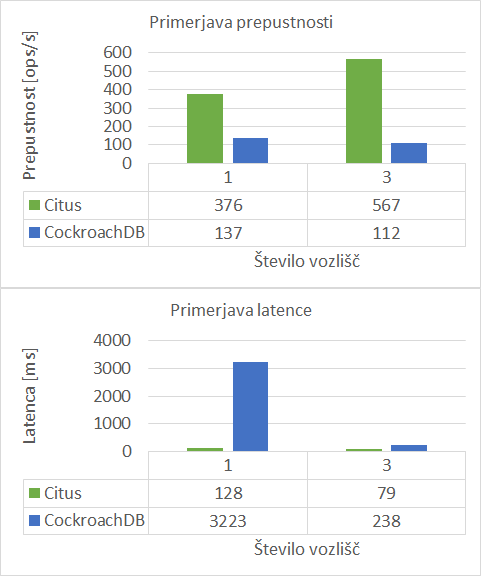
\includegraphics[width=0.7\textwidth]{resources/top-level-comparison.png}
\end{center}
\caption{Groba primerjava povprečne prepustnosti in latence med obema podatkovnima bazama na enem in treh vozliščih. \DIFdelbeginFL \DIFdelFL{Z }\DIFdelendFL \DIFaddbeginFL \DIFaddFL{Iz }\DIFaddendFL grafov je razvidno, da podatkovna baza CockroachDB dosega bistveno manjšo prepustnost\DIFaddbeginFL \DIFaddFL{, }\DIFaddendFL poleg tega pa ima večjo latenco.}
\label{img_ycsb_results_top_level_comparison}
\end{figure}

\newpage

\begin{figure}[H]
\begin{center}
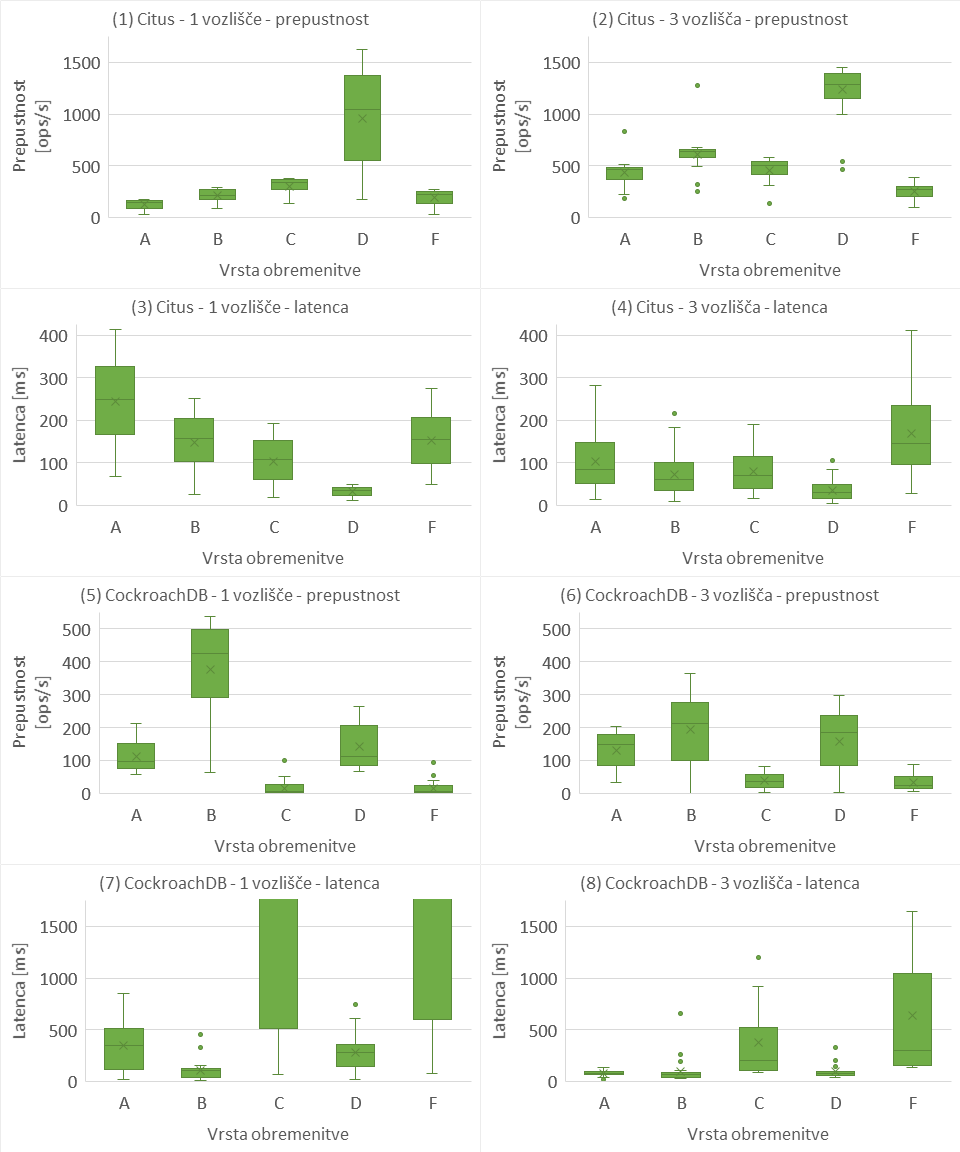
\includegraphics[width=1\textwidth]{resources/comparison-throughputnlatency-bnw.png}
\end{center}
\caption{Prikazuje primerjavo prepustnosti in latenc glede na vrsto obremenitve med podatkovno bazo Citus in CockroachDB. Graf (7) je zaradi lažje primerjave odrezan. \DIFdelbeginFL \DIFdelFL{Z }\DIFdelendFL \DIFaddbeginFL \DIFaddFL{Iz }\DIFaddendFL grafov \DIFdelbeginFL \DIFdelFL{se vidi}\DIFdelendFL \DIFaddbeginFL \DIFaddFL{je razvidno}\DIFaddendFL , da je podatkovna baza Citus v primerjavi \DIFdelbeginFL \DIFdelFL{z }\DIFdelendFL \DIFaddbeginFL \DIFaddFL{s }\DIFaddendFL CockroachDB veliko bolj stabilna, kar se odraža v razponu med največjo in najmanjšo vrednostjo.}
\label{img_ycsb_results_bnw_comparison}
\end{figure}

\newpage

\begin{figure}[H]
\begin{center}
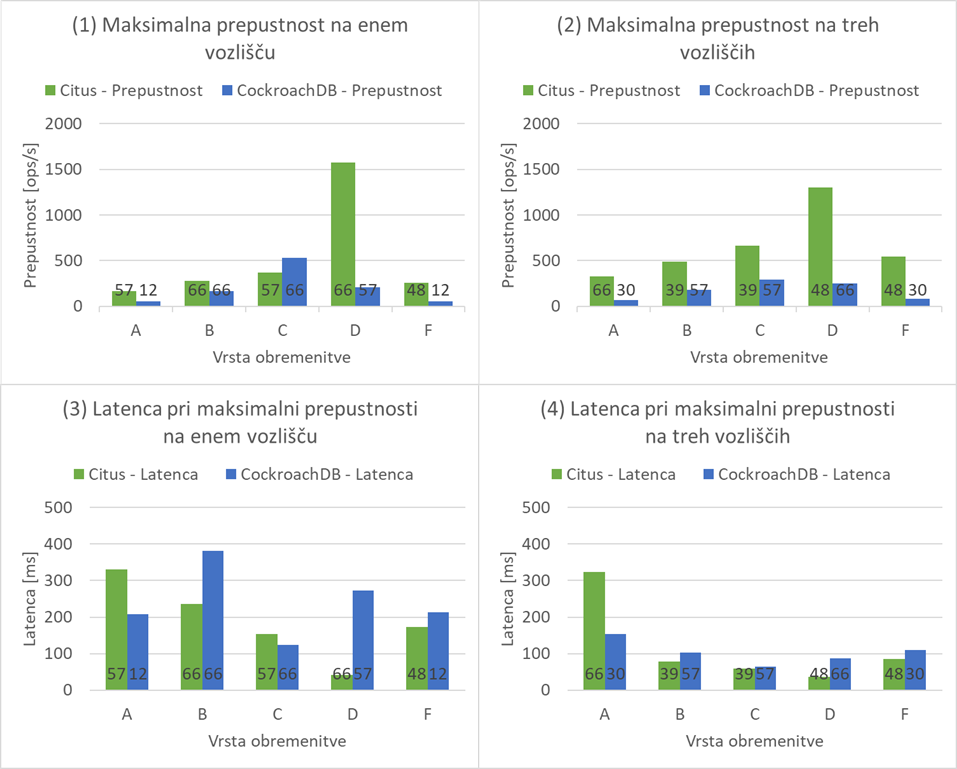
\includegraphics[width=1.0\textwidth]{resources/maxThroughput.png}
\end{center}
\caption{Prikazuje primerjavo prepustnosti in latence za vzorec z \DIFdelbeginFL \DIFdelFL{maksimalna prepustnost}\DIFdelendFL \DIFaddbeginFL \DIFaddFL{maksimalno prepustnostjo}\DIFaddendFL . Številke v spodnjem delu serije predstavljajo število sočasnih niti, pri katerih je bila dosežena maksimalna prepustnost. \DIFdelbeginFL \DIFdelFL{Z }\DIFdelendFL \DIFaddbeginFL \DIFaddFL{Iz }\DIFaddendFL grafov lahko razberemo, da se podatkovna baza CockroachDB z vidika sočasnih obremenitev skalira bolje kot Citus.}
\label{img_ycsb_results_max_throughput}
\end{figure}

\newpage

\section{Ugotovitve}
Zmogljivostna analiza je pokazala, da se podatkovna baza Citus pri večini obremenitev, katere \DIFdelbegin \DIFdel{sem testiral, odziva bitveno }\DIFdelend \DIFaddbegin \DIFadd{smo testirali, odziva bistveno }\DIFaddend bolje kot podatkovna baza CockroachDB.

S slike \ref{img_ycsb_results_top_level_comparison} je razvidno, da CockroachDB v primerjavi s Citus dosega 2,\DIFdelbegin \DIFdel{7 krat }\DIFdelend \DIFaddbegin \DIFadd{7-krat }\DIFaddend manjšo prepustnost na enem vozlišču in kar \DIFdelbegin \DIFdel{5 krat }\DIFdelend \DIFaddbegin \DIFadd{5-krat }\DIFaddend manjšo prepustnost na treh vozliščih. Pri primerjavi latence pa je CockroachDB v primerjavi s Citus na enem vozlišču dosegel približno 25,\DIFdelbegin \DIFdel{2 krat }\DIFdelend \DIFaddbegin \DIFadd{2-krat }\DIFaddend večjo latenco, na treh vozliščih pa samo še \DIFdelbegin \DIFdel{3 krat }\DIFdelend \DIFaddbegin \DIFadd{3-krat }\DIFaddend večjo.

S slike \ref{img_ycsb_results_bnw_comparison} je razvidno, da je podatkovna baza CockroachDB v primerjavi s podatkovno bazo Citus manj stabilna. To se odraža na posameznih grafih\DIFaddbegin \DIFadd{, }\DIFaddend saj so podatki pri podatkovni bazi CockroachDB veliko bolj razpršeni.

Če primerjamo spremembe sočasnih niti, pri katerih sta bazi dosegali maksimalno prepustnost (slika \ref{img_ycsb_results_max_throughput})\DIFaddbegin \DIFadd{, }\DIFaddend opazimo naslednje. Podatkovna baza CockroachDB ob skaliranju na tri vozlišča \DIFaddbegin \DIFadd{lahko }\DIFaddend v povprečju \DIFdelbegin \DIFdel{lahko }\DIFdelend obdela 5,4 več sočasnih niti, podatkovna baza Citus pa kar 10,8 manj.

\subsection{Hipoteza 1}
\textit{CockroachDB bo na enem vozlišču nekoliko počasnejši od PostgreSQL podatkovne baze.}

\ \\
Razlog za to hipotezo je, da je podatkovna baza PostgreSQL že dolgo na trgu \cite{Postgres-first-release} in je uporabljena na mnogih projektih. Zato je zmogljivostno bolje optimizirana\DIFaddbegin \DIFadd{, }\DIFaddend kakor CockroachDB. CockroachDB pa je na trgu od leta 2015. Prvo stabilno verzijo (1.0.0) so objavili maja 2017 \cite{CRDB-2017}, druga verzija (2.0.0) pa je bila objavljena aprila 2018. Vsaka verzija je dodala veliko novih funkcionalnosti.

% \begin{figure}[H]
% \begin{center}
% 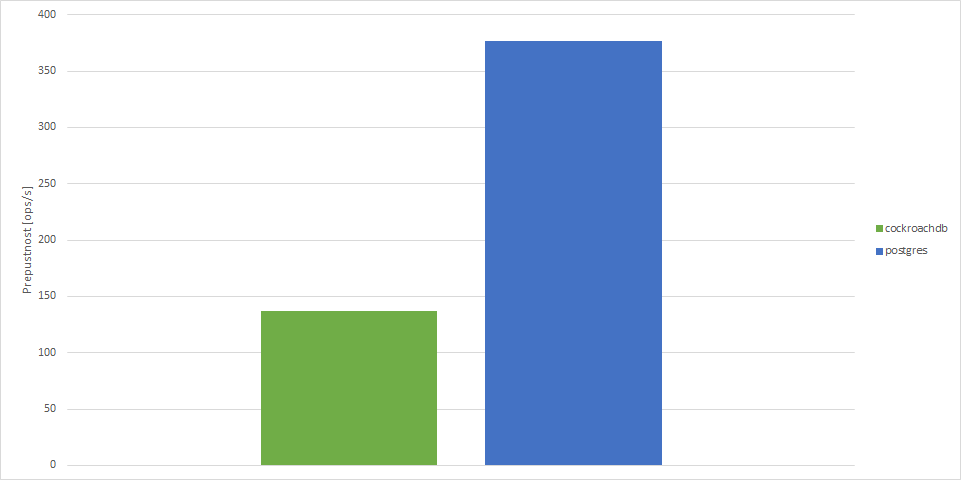
\includegraphics[width=1\textwidth]{resources/throughput-comparison-n1-v2.png}
% \end{center}
% \caption{Primerjava povprečne prepustnosti na enem vozlišču.}
% \label{img_ycsb_results_throughptu_comparison_n1}
% \end{figure}

Hipotezo \DIFdelbegin \DIFdel{sem potrdil}\DIFdelend \DIFaddbegin \DIFadd{smo potrdili}\DIFaddend , kar je razvidno tudi na sliki \ref{img_ycsb_results_top_level_comparison}. Podatkovna baza CockroachDB v primerjavi \DIFdelbegin \DIFdel{z }\DIFdelend \DIFaddbegin \DIFadd{s }\DIFaddend PostgreSQL dosega približno 2,\DIFdelbegin \DIFdel{7 krat }\DIFdelend \DIFaddbegin \DIFadd{7-krat }\DIFaddend nižjo prepustnost.

Podobno zmogljivostno primerjavo so decembra 2017 izvedli na zasebni raziskovalni univerzi v Bruslju \cite{CRDB-2017}. Z orodjem YCSB (verzija 0.12.0) so primerjali obremenitve tipa A, B in C. Ugotovili so, da se podatkovna baza CockroachDB (verzija 1.1.3) v primerjavi \DIFdelbegin \DIFdel{z }\DIFdelend \DIFaddbegin \DIFadd{s }\DIFaddend PostgreSQL (verzija 9.6.5) odziva približno \DIFdelbegin \DIFdel{10 krat }\DIFdelend \DIFaddbegin \DIFadd{10-krat }\DIFaddend slabše\DIFaddbegin \DIFadd{, }\DIFaddend kakor PostgreSQL. V njihovem primeru so testno okolje postavili v Amazon oblaku, vsako bazo na treh vozliščih.

\subsection{Hipoteza 2}
\textit{CockroachDB bo zaradi linearne skalabilnosti na treh vozliščih skoraj \DIFdelbegin \DIFdel{tri krat }\DIFdelend \DIFaddbegin \DIFadd{3-krat }\DIFaddend bolj zmogljiv.}

\ \\
Vsa vozlišča\DIFaddbegin \DIFadd{, }\DIFaddend povezana v CockroachDB gručo\DIFaddbegin \DIFadd{, }\DIFaddend so simetrična, kar pomeni, da vsa vozlišča opravljajo enake naloge. Ob predpostavki, da se uporabniki enakomerno razporedijo preko vseh vozlišč, ter \DIFdelbegin \DIFdel{, }\DIFdelend da je obremenitev enakomerna, naj bi bila rast prepustnosti linearna \cite{CRDB-design}.

% \begin{figure}[H]
% \begin{center}
% 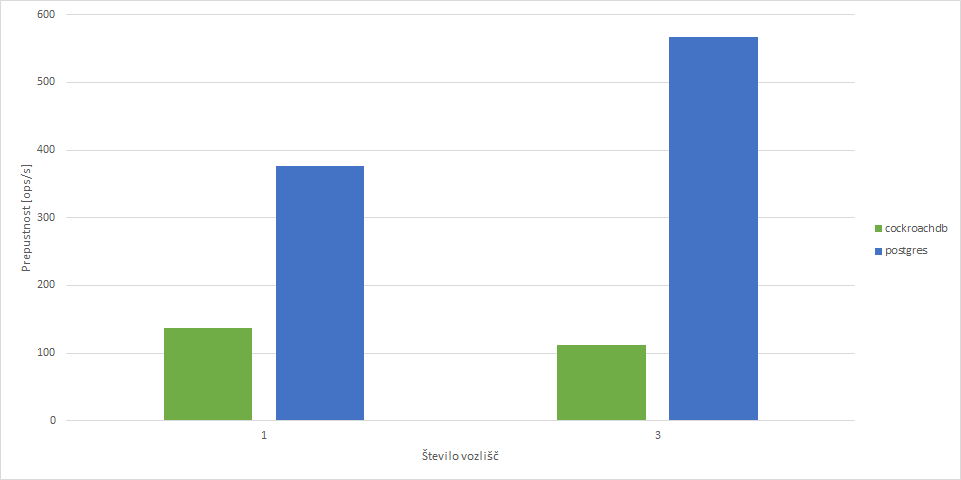
\includegraphics[width=1\textwidth]{resources/scaling-throughput-v2.png}
% \end{center}
% \caption{Primerjava povprečne prepustnosti ob skaliranju baze na tri vozlišča.}
% \label{img_ycsb_results_scaling_throughptu_comparison}
% \end{figure}

To hipotezo \DIFdelbegin \DIFdel{sem ovrgel}\DIFdelend \DIFaddbegin \DIFadd{smo ovrgli}\DIFaddend . Meritve so pokazale, da podatkovna baza CockroachDB doseže celo slabšo prepustnost na treh vozliščih. To \DIFdelbegin \DIFdel{razvidno na sliki }\DIFdelend \DIFaddbegin \DIFadd{je razvidno iz slike }\DIFaddend \ref{img_ycsb_results_top_level_comparison}.

Razlog za tak rezultat naj bi bila primerjava med konfiguracijo na enem in treh vozliščih \cite{CRDB-YCSB-perf-analisis}. CockroachDB na treh vozliščih s privzetimi nastavitvami začne \DIFdelbegin \DIFdel{z }\DIFdelend \DIFaddbegin \DIFadd{s }\DIFaddend postopkom replikacije podatkov. Privzeto je vsak podatek repliciran trikrat, enkrat na vsakem vozlišču. CockroachDB tako zagotavlja konsistenco in visoko razpoložljivost.

Rezultati neuradne TPC-C zmogljivostne analize, katero so izvedli v Co\-ckroachLabs, kažejo, da je CockroachDB linearno skalabilen \cite{CRDB-TPCC-perforamance-report}. Ob skali\-ranju \DIFdelbegin \DIFdel{z }\DIFdelend \DIFaddbegin \DIFadd{iz }\DIFaddend 3 na 30 vozlišč ter ob sorazmernem povečanju obremenitve so dosegli tudi sorazmerno večjo prepustnost.

\DIFdelbegin \DIFdel{Prišel sem }\DIFdelend \DIFaddbegin \DIFadd{Prišli smo }\DIFaddend do ugotovitve, da je CockroachDB linearno skalabilna podatkovna baza \DIFdelbegin \DIFdel{, }\DIFdelend (1)\DIFaddbegin \DIFadd{, }\DIFaddend če je obremenitev enakomerno porazdeljena med vsa vozlišča in (2) faktor replikacije ob skaliranju ostane konstanten.

Na podlagi teh ugotovitev \DIFdelbegin \DIFdel{sem pripravil }\DIFdelend \DIFaddbegin \DIFadd{smo pripravili }\DIFaddend optimistično oceno rasti povprečne prepustnosti. Obe bazi se v idealnih pogojih in do neke mere skalirata linearno, kar je prikazano na sliki \ref{img_ycsb_results_scaling_throughptu_prediction}. Vendar pa se pri PostgreSQL konfiguraciji vsi odjemalci \DIFdelbegin \DIFdel{direktno }\DIFdelend \DIFaddbegin \DIFadd{neposredno }\DIFaddend povezujejo na eno vozlišče (koordinatorja), \DIFdelbegin \DIFdel{to vozlišče }\DIFdelend \DIFaddbegin \DIFadd{ki }\DIFaddend je ozko grlo (točka A), saj bo ob \DIFdelbegin \DIFdel{večanjem }\DIFdelend \DIFaddbegin \DIFadd{večanju }\DIFaddend v neki točki prišlo do zasičenosti resursov \cite{Citus-add-coordinator}. V neki točki (točka B) pa bo CockroachDB presegel prepustnost podatkovne baze Citus.

\begin{figure}[H]
\begin{center}
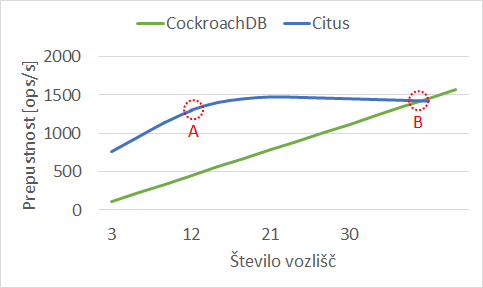
\includegraphics[width=1\textwidth]{resources/scaling-throughput-prediction-v2.png}
\end{center}
\caption{Optimistična ocena rasti povprečne prepustnosti. Pri podatkovni bazi Citus \DIFdelbeginFL \DIFdelFL{, }\DIFdelendFL se v točki A linearna rast konča. V točki B pa \DIFdelbeginFL \DIFdelFL{je }\DIFdelendFL ima CockroachDB že večjo prepustnost. Graf je le simboličen in ne predstavlja realnih meritev.}
\label{img_ycsb_results_scaling_throughptu_prediction}
\end{figure}


\chapter{Sklepne ugotovitve}

V diplomskem delu smo pregledali lastnosti  ter najpogosteje uporabljene mehanizme in pristope pri implementacijah novih arhitektur NewSQL podatkovnih baz. Opisali smo arhitekturo in lastnosti izbrane NewSQL podatkovne baze CockroachDB \cite{CRDB-home}. Podatkovno bazo CockroachDB smo kasneje praktično testirali. \DIFdelbegin \DIFdel{Izvedeli }\DIFdelend \DIFaddbegin \DIFadd{Izvedli }\DIFaddend smo primerjalno analizo zmogljivosti med podatkovno bazo CockroachDB in PostgreSQL \cite{postgres} (z nameščeno razširitvijo Citus \cite{citus}). Veliko časa smo vložili v postavitev testnega okolja in bili pozorni, da smo odpravili čim več spremenljivk, ki bi lahko vplivale na testne scenarije. Testno okolje je bilo sestavljeno \DIFdelbegin \DIFdel{s }\DIFdelend \DIFaddbegin \DIFadd{iz }\DIFaddend štirih starejših računalnikov, \DIFdelbegin \DIFdel{kateri }\DIFdelend \DIFaddbegin \DIFadd{ki }\DIFaddend so bili povezani preko gigabitnega omrežja, na njih pa je tekel Ubuntu Server \cite{ubuntu-server} in Docker \cite{docker}. Testno okolje smo v začetku nadzirali preko Telegraf agenta \cite{telegraf}, InfluxDB podatkovne baze za shranjevanje časovnih podatkov \cite{influxdb} in Grafane za vizualizacijo podatkov \cite{grafana}. Kljub trudu, ki smo ga vložili v postavitev testnega okolja, bi \DIFdelbegin \DIFdel{le }\DIFdelend tega lahko še izboljšali. Za boljšo primerljivost zmogljivostnih metrik \DIFdelbegin \DIFdel{, }\DIFdelend bi morala imeti vsa vozlišča enako strojno opremo, testirati pa bi moral še konfiguracije z več kot tremi vozlišči. Izvedbo testiranja smo avtomatizirali. Z orodjem YCSB \cite{brianfrankcooper/YCSB} smo izvajali različne zmogljivostne teste, rezultate pa shranjevali v CSV datoteko in jih kasneje analizirali.

Primerjalna analiza zmogljivosti je pokazala, da je podatkovna baza Cock\-roachDB kljub enostavnim obremenitvam, katere vrši orodje YCSB, v večini primerov bistveno slabša od PostgreSQL podatkovne baze. V povprečju je imela podatkovna baza Cock\-roachDB \DIFdelbegin \DIFdel{3 krat }\DIFdelend \DIFaddbegin \DIFadd{3-krat }\DIFaddend večjo latenco in \DIFdelbegin \DIFdel{5 krat }\DIFdelend \DIFaddbegin \DIFadd{5-krat }\DIFaddend manjšo prepustnost kakor podatkovna baza PostgreSQL na treh vozliščih.
% Poleg tega pa je z večanjem sočasnih povezav zmogljivost padala bistveno hitreje kot pri podatkovni bazi PostgreSQL.
Kljub slabšim rezultatom zmogljivostne analize \DIFdelbegin \DIFdel{, }\DIFdelend se moramo zavedati, da je težko pošteno primerjati dve zelo različni podatkovni bazi. Podatkovna baza PostgreSQL je bistveno starejša in zato bolj stabilna ter optimizirana. CockroachDB pa je na trgu šele dobri dve leti in je trenutno še vedno bolj funkcionalno usmerjena. Za smiselno odločitev pri izbiri podatkovne baze moramo poleg zmogljivostnih metrik upoštevati tudi druge, kot so poizvedovalni jezik, podpora transakcijam, zrelost sistema, skupnost, zmogljivost, težavnost postavitve ter vzdrževanja, ostale lastnosti\DIFaddbegin \DIFadd{, }\DIFaddend specifične za vsako podatkovno bazo \DIFdelbegin \DIFdel{, }\DIFdelend ...

Podatkovna baza CockroachDB ima močno in aktivno skupnost. Na spletu najdemo že kar nekaj vrednotenj drugih avtorjev, od raznih primerjalnih analiz \cite{kaur2017performance, Benchmarking-GCS-CRDB-NuoDB, CRDB-tpcc-vs-aurora, CRDB-2017}, do Jepsen testov konsistence in obnašanja sistema med napakami \cite{CRDB-jepsen, CRDB-jepsen-diy}.

Kljub temu, da je CockroachDB relativno nova podatkovna baza, jo podjeta že uporabljajo. Na primer podjetje Baidu \cite{crdb-baidu} \DIFdelbegin \DIFdel{, }\DIFdelend uporablja CockroachDB pri dveh novih aplikacijah, ki sta predhodno uporabljale MySQL podatkovno bazo. Ti dve aplikaciji obsegata približno \DIFdelbegin \DIFdel{2TB }\DIFdelend \DIFaddbegin \DIFadd{2 TB }\DIFaddend podatkov in ustvarita približno \DIFdelbegin \DIFdel{50M }\DIFdelend \DIFaddbegin \DIFadd{50 M }\DIFaddend zapisov na dan. Podjetje Kindred \cite{crdb-kindred} \DIFdelbegin \DIFdel{, ki se ukvarja z }\DIFdelend \DIFaddbegin \DIFadd{se ukvarja s }\DIFaddend spletnim igralništvom\DIFdelbegin \DIFdel{. Z }\DIFdelend \DIFaddbegin \DIFadd{, z }\DIFaddend letom 2014 pa so začeli s prehodom na globalni trg. Imajo kompleksen ekosistem z več kot 200 \DIFdelbegin \DIFdel{mikrostoritev}\DIFdelend \DIFaddbegin \DIFadd{mikrostoritvami}\DIFaddend . Ta arhitektura omogoča elastičnost\DIFaddbegin \DIFadd{, }\DIFaddend vendar pa mora biti skoraj v celoti avtonomna. CockroachLabs poizkuša s podjetji sodelovati, nekatera podjetja so tudi prispevala del funkcionalnosti. Podjetja\DIFaddbegin \DIFadd{, }\DIFaddend katera so se odločila za uporabo podatkovne baze CockroachDB, ciljajo globalni trg, poleg tega pa želijo poenostaviti postavitev in vzdrževanje, tako v \DIFdelbegin \DIFdel{oblak, kako }\DIFdelend \DIFaddbegin \DIFadd{oblaku, kakor }\DIFaddend tudi na svoji infrastrukturi.

Glede na znanje\DIFdelbegin \DIFdel{katerega smo pridobil }\DIFdelend \DIFaddbegin \DIFadd{, katerega smo pridobili }\DIFaddend skozi diplomsko delo, menimo, da je podatkovna baza CockroachDB primerna za nove transakcijsko usmerjene (OLTP) aplikacije, katere zahtevajo konsistenco in \DIFdelbegin \DIFdel{visko }\DIFdelend \DIFaddbegin \DIFadd{visoko }\DIFaddend razpoložljivost\DIFaddbegin \DIFadd{, }\DIFaddend hkrati pa ciljajo hitrorastoč globalni trg \DIFdelbegin \DIFdel{. Za aplikacije}\DIFdelend \DIFaddbegin \DIFadd{ter za aplikacije, }\DIFaddend kjer je čas do trga zelo pomemben in kjer si ne moremo privoščiti velikih stroškov vzdrževanja. Pred odločitvijo moramo oceniti še podprto sintakso SQL jezika \cite{CRDB-sql-features} in morebitne ostale lastnosti \cite{CRDB-limitations}. Podatkovna baza CockroachDB trenutno ni primerna za scenarije\DIFdelbegin \DIFdel{kateri }\DIFdelend \DIFaddbegin \DIFadd{, ki }\DIFaddend zahtevajo kompleksne stične operacije, nizko latenco in analitično usmerjene aplikacije (OLAP) \cite{CRDB-FAQ}.

V prihodnje bi bilo zanimivo raziskati in primerjati še zelo podobno in prav tako odprtokodno podatkovno bazo TiDB \cite{PingCAP-home}. TiDB je trenutno še zelo mlad produkt, z verzijo 1.0.0, ki je izšla sredi oktobra 2017\DIFaddbegin \DIFadd{, }\DIFaddend in verzijo 2.0.0 iz aprila 2018. TiDB prav tako idejno temelji na podatkovni bazi Google Spanner in se v nekaterih arhitekturnih lastnostih zelo ujema s podatkovno bazo CockroachDB. Najbolj očitna razlika je, da je arhitektura ločena na tri večje komponente, poleg tega za sinhronizacijo ure uporablja drugačen pristop. Razvijalci podatkovne baze TiDB obljubljajo, da je podatkovna baza primerna za hibridne transakcijske in analitične obremenitve.

Zanimivo bi bilo tudi razširiti zmogljivostno primerjalno analizo\DIFdelbegin \DIFdel{izvedeno v tej diplomski nalogi}\DIFdelend \DIFaddbegin \DIFadd{, izvedeno v tem diplomskem delu}\DIFaddend . Porazdeljene podatkovne baze\DIFaddbegin \DIFadd{, }\DIFaddend kot je CockroachDB\DIFaddbegin \DIFadd{, }\DIFaddend so primerne za okolja z vsaj tremi vozlišči\DIFdelbegin \DIFdel{, zanimivo }\DIFdelend \DIFaddbegin \DIFadd{. Zanimivo }\DIFaddend bi bilo ugotoviti\DIFaddbegin \DIFadd{, }\DIFaddend kaj se dogaja, ko v gručo povežemo še več vozlišč. Poleg osnovnih YCSB obremenitev \DIFdelbegin \DIFdel{, }\DIFdelend bi bilo zanimivo preveriti še druge, kot sta TPC-C in TPC-H.


\newpage %dodaj po potrebi, da bo številka strani za Literaturo v Kazalu pravilna!
\ \\
\clearpage
\addcontentsline{toc}{chapter}{Literatura}
\bibliographystyle{plain}
\bibliography{bibliography}


\end{document}

